%*****************************************
\chapter{Bestehende Systeme}\label{ch:research}
%*****************************************
In der Arbeitswelt kommt es immer wieder zu Situationen, in der sich mehrere Personen treffen um zusammen Probleme zu diskutieren. Statistiken besagen, dass Büroangestellte sogar bis zu 70 Prozent ihrer Arbeitszeit in Meetings verbringen \citep{panko:1993}. Die meisten Meetings werden mit Hilfsmittel wie Whiteboards, Flipcharts oder Notizblöcke abgehalten, da meistens Notierungsbedarf bei neuen Ideen, Problemlösungen etc. besteht. Computer können dabei sehr hilfreich sein, wäre da nicht die Hürde der Dateneingabe die zu bewältigen ist. Herkömmliche Eingaben via Maus und Tastatur verlangsamen den natürlichen explorativen Charakter eines Meetings. Elektronische Skizzierwerkzeuge inklusive gemeinsam verwendbarer Zeichenoberflächen können hier Abhilfe für kollaboratives Arbeiten schaffen. 

\medskip Das folgende Kapitel soll anhand von Beispielen und Projekten aus der Literatur zeigen, durch welche Methoden Meetings bzw. im speziellen Designsessions unterstützt werden können. Besonderer Augenmerk soll dabei auf das Skizzieren als Designmethode und kooperatives Arbeiten in CSCW\footnote{Computer Supported Cooperative Work} Umgebungen liegen.

\section{Arbeitsweisen von Designteams}
Um herauszufinden mit welchen Methoden oder Werkzeugen man kollaborative Meetings und im Zuge dessen den Designprozess unterstützen kann, muss man zuerst wissen wie Designer zusammen arbeiten. John Tang und Larry Leifer versuchten in \citep{Tang:1988p279} als Teil einer Studie, mittels empirischen Daten das Verhalten von Designern in Meetings zu untersuchen. Dazu bildeten sie ein Framework und konzentrierten sich auf deren Arbeitsaktivitäten wie \emph{Auflisten}, \emph{Zeichnen} und \emph{Gestikulieren}, welche sie den zugehörigen Kontext zuordneten. Um diesen einzuschränken, bildeten sie vier Funktionen, die den Hauptzweck der Aktivitäten beschreiben: \emph{Festhalten von Informationen}, \emph{Vermitteln von Ideen}, \emph{Darstellen von Ideen} und \emph{Erlangen von Aufmerksamkeit}. In einem Framework (siehe \autoref{fig:tangFramework}) stellten sie diese gegenüber und verwendeten die Daten zur Auswertung.

\medskip Obwohl sich Tang und Leifer mit ihrer Arbeit gezielt auf den Designprozess zubewegen, erwarten sie dadurch auch relevante Ergebnisse für kollaboratives Arbeiten im Allgemeinen. \par Kollaboratives Arbeiten ist für Designer eine gängige Art Probleme anzugehen und kann von den sonstigen individuellen Aktivitäten deutlich abgegrenzt werden, wie auch frühere empirische Designstudien bestätigen können: \citep{Ullman:1987, Ballay:1987, Akin:1978, Lera:1983}.

\medskip In ihrer Studie führten sie 8 Sessions mit Teams zu je 3-4 Personen durch, welche jeweils eineinhalb Stunden dauerten. Die Gruppen trafen sich dafür in Konferenzräumen und saßen um einen Tisch mit einem großen Bogen Papier als Schreibunterlage. Jede Gruppe arbeitete zwar an einer anderen Designaufgabe, jedoch waren alle Teil des Designs eines Mensch-Maschinen Interfaces für ein >>smartes<< (Mikroprozessor gesteuertes) Gerät.
Die Analyse der Tests wurde durch das NoteCards Hypertext Environment \citep{Halasz:1986:NN:29933.30859} erheblich vereinfacht. Das System half die Daten zu strukturieren und aufzubereiten. \autoref{fig:tangTranskript} zeigt einen Auszug des Transkripts der ersten Session mit Anmerkungen zu einzelnen Aktivitäten und einen Teil der Schreibunterlage, welche die dazu erstellte Skizze beinhaltet. Jede Aktivität wurde anhand der Funktionen des Frameworks kategorisiert und abgezählt, um in Folge dessen die Daten statistisch auszuwerten. \autoref{fig:tangStatistik} veranschaulicht die Ergebnisse.

\medskip Wie die Abbildung zeigt, sind knapp die Hälfte (46\%) aller Aktivitäten von illustrativen Charakter, was die Wichtigkeit von Skizzen belegt. Zusätzlich kommt der Vermittlung und Darstellung von Ideen (zusammen 43\%) auch große Bedeutung zu.\par
\medskip \emph{Anmerkung: \graffito{\(\clubsuit\)} An diesem Punkt der Arbeit soll noch nicht auf die gesamten Erkenntnisse der Analyse eingegangen werden, sondern lediglich auf die der Ideenentwicklung. Die weiteren Ergebnisse werden in den Kapiteln \nameref{ch:SingleVSGroupDesign} und \nameref{ch:CSCWDesign} behandelt.}

\medskip Die Schreibunterlage spielt im Prozess der Ideenentwicklung, neben der des Festhaltens von Informationen und der Vermittlung von Ideen, eine aktive Rolle. Die Unterstützung dieses Prozesses (zb. durch elektronische Hilfsmittel) ist aber alles andere als unproblematisch, wie beispielsweise die Frustrationen von Designer beweisen, die versuchen konventionelle CAD Tools für die Weiterentwicklung von Ideen - von konzeptionellen Skizzen zu formellen Spezifikationen - zu verwenden. Dieser Aspekt zeigt die Verwendung der Schreibunterlage als Teil eines interaktiven Prozesses, anstatt der Reduzierung dessen auf ein Text-Grafik Artefakt. 

%\clearpage
\begin{figure}
        {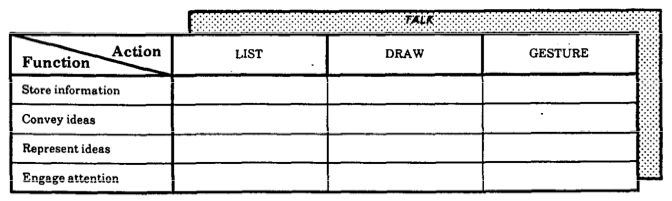
\includegraphics[width=1\linewidth]{gfx/tangFramework}}
		\caption[Framework zur Untersuchung von Designaktivitäten.]{Das Framework zur Untersuchung von Designaktivitäten. In ihm werden die Aktivitäten den zweckmäßigen Funktionen gegenübergestellt. Es dient als empirische Grundlage. }\label{fig:tangFramework}
\end{figure} 

\begin{figure}[bth]
        \myfloatalign
        \subfloat[Transkriptauszug]
        {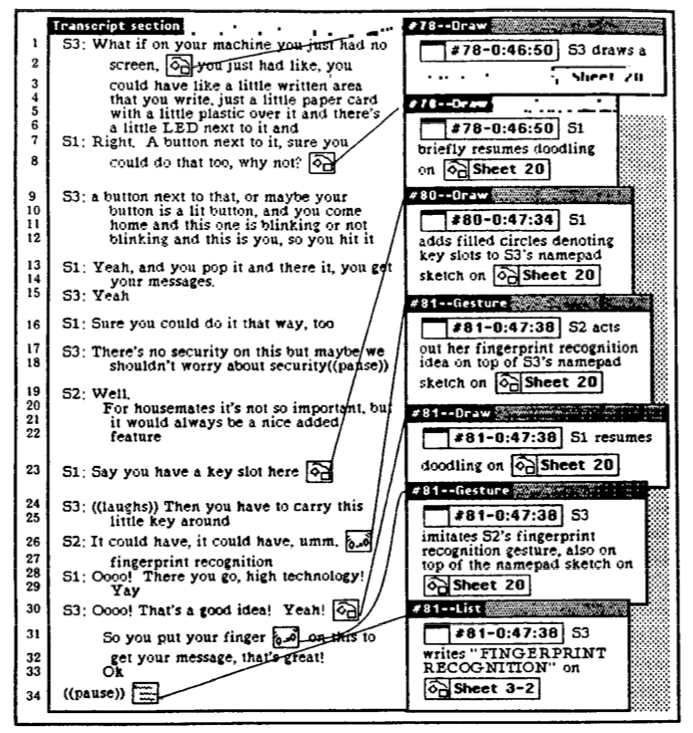
\includegraphics[width=.65\linewidth]{gfx/tangTranskript}} \quad
        \subfloat[Artefakt]
        {\label{fig:tangTranskriptB}%
         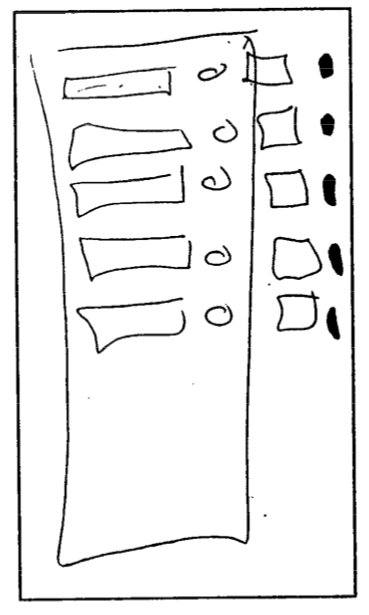
\includegraphics[width=.25\linewidth]{gfx/tangTranskriptB}} \\
        \caption[Auszug des Transkripts inklusive dazugehöriges angefertigtes Artefakt der ersten Designsession.]{Ein Auszug des Transkripts, erstellt mit Hilfe von NoteCards \citep{Halasz:1986:NN:29933.30859}, inklusive dazugehörigen  Artefakt der ersten Designsession. Es zeigt wie jeder Teilnehmer in kürzester Zeit einen eigenen Gedanken äußert und diesen im Artefakt manifestiert.}\label{fig:tangTranskript}
\end{figure}

\begin{figure}
        {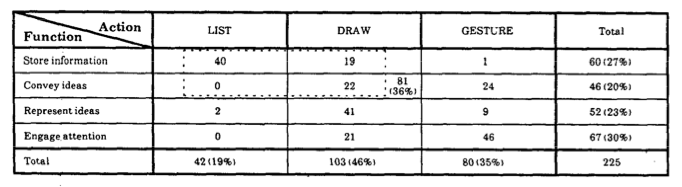
\includegraphics[width=1\linewidth]{gfx/tangStatistik}}
		\caption[Statistische Ergebnisse der ersten Designsession.]{Statistische Ergebnisse der ersten Designsession. Alle Aktivitäten wurden dafür im Framework anhand der Funktionen kategorisiert und anschließend abgezählt.}\label{fig:tangStatistik}
\end{figure}
\clearpage

\medskip Die Studie beobachtete zwei Schlüsselmerkmale, auf die Designer bei der Entwicklung von Ideen zurückgriffen: a) In der Lage sein ohne Weiteres Darstellungen von Ideen auf einer Schreibunterlage auszuprobieren, und b) diese Darstellungen stufenweise in genaue Artefakte weiterzuverarbeiten - oft durch die Zusammenarbeit mit anderen Partizipienten. \citep{Tang:1988p279}

\medskip Gemeinsam verwendbare Zeichenoberflächen spielen auch laut Sara Bly \citep{Bly:1988:UDS:62266.62286} eine besonders wichtige Rolle in Designsessions mit mehreren Teilnehmern. 
Bly beobachtete das Skizzierverhalten zweier Personen in Face-to-Face Designsessions und zeichnete diese für spätere Anaylsen auf Video auf. Bei der Auswertung stellte sie fest, dass nahezu die Hälfte aller Aktivitäten, in denen Gebrauch von Schreibwerkzeugen gemacht wurde, Skizzen waren. Noch interessanter war aber die Tatsache, dass sich im Laufe der Session verschiedene Zeichenbereiche herauskristallisiert haben. So entstanden einzelne Bereiche in denen nur ein Designer gezeichnet hat und Bereiche die zusammen benutzt wurden. 78\% aller Aktivitäten fanden jedoch im gemeinsamen Bereich statt und 25\% aller Aktivitäten eines Designers entstanden im Anschluss zu einer Zeichnung eines anderen Designers. Die Analyse zeigt also die Wichtigkeit von gemeinsamen Bereichen in Designsessions mit mehreren Teilnehmern. Zusätzlich spielten Gesten und Betonungen in Erläuterungen eine wichtige Rolle, welche die Notwendigkeit der physischen Anwesenheit nahelegt.

\section{Skizziertools in kooperativen Settings}

%Brainstormingsessions in Meetings sind ein wesentlicher Teil des Designprozesses. Typischer Weise fungiert dabei ein Teilnehmer der Gruppe als >>Schreiber<< und %fördert die Gruppendiskussion durch Notizen auf einem Whiteboard. Die anderen Teilnehmer sitzen um das Whiteboard mit eigenen Notitzbüchern und schreiben zusätzliche %persönliche Anmerkungen. Das Whiteboard spielt eine wichtige Rolle in der Vermittlung der Gruppeninteraktionen, durch Richten des Augenmerks auf eine große gemeinsam %genutzte Anzeige. Das Skizzieren am Whiteboard ist ein wichtger Part der Brainstormingaktivität, da - wie auch Forschung belegt - Skizzieren die Gruppenkommunikation %und den Prozess der Ideengenerierung fördert. \citep{Tang1991143} Skizzieren unterstützt wiederholt interpretierende Denkzyklen und den Zugang zu anfänglichen Ideen %\citep{vanDerLugt:2002}. 

Tools und Umgebungen herkömmlicher Brainstormingmeetings besitzen zwar physikalische Qualitäten, unterstützen jedoch nur unausreichend gemeinsames Zeichnen mehrerer Personen. Gleichzeitiges Arbeiten an einer Skizze, z.B. am Whiteboard, ist heikel, da Personen nahe beisammen stehen müssen und sich gegenseitig oft im Weg sind. Es ist physikalisch unmöglich an der exakt selben Stelle der Tafel zu arbeiten. Tang spricht hier von einem eindeutigen Bedarf an einem gleichzeitigen Zugriff auf die Arbeitsfläche in kollaborativen Gruppenmeetings \citep{Tang1991143}.

Über die Jahre wurden einige Versuche gestartet diesen Wunsch mit Hilfe von elektronischen Mitteln nach zu kommen. Im folgenden will ich nun einige davon beschreiben.
%Zusätzlich beobachteten Bastéa-Forte und Yen (\citep{Bastea-Forte:2007}), dass sitzende Teilnehmer ungern aufstehen um sich einem Whiteboard zu nähern. In vielen Fällen, wenn eine beschriebene Idee nicht verstanden wird, müssen sitzende Teilnehmer explizit gebeten werden zum Whiteboard zu gehen um die Idee aufzuzeichnen. Dadurch schreibt meistens nur eine Person auf das Whiteboard, was das Ergebnis des Geschriebenen und die Art wie es geschrieben wird verfälscht. Digitale Whiteboards bringen hingegen die Vorteile einer automatischen Dokumentation und der Anzeige von externen Bildern. 
% -------

\subsection{XSketch}
Bereits 1990 nahm sich das Department of Computer Science an der Universität in Toronto Tangs und Blys Arbeiten als Ansporn bzw. Grundlage für weitere Arbeiten und entwickelte \emph{XSketch}: ein multi-user Skizzierwerkzeug für X11\footnote{X11 ist ein Softwaresystem für UNIX Plattformen, dass ein Grafisches User Interface (GUI) zur Verfügung stellt - auch bekannt als X-Windows.}, dass Jefferey J. Lee in \citep{Lee:1990:XMS:91478.91510} vorstellt.

\medskip Die Grundidee von \emph{XSketch} ist ein simples Werkzeug für multi-user Design- und Brainstormingsessions bereitzustellen. Da es aber auch für einzelne Benutzer geeignet sein soll, hat der Multi-user-Faktor nur wenig Einfluss auf das User Interface. Es setzt auf eine Server-Client Architektur, in der alle Nachrichten und Entscheidungen zentral gesteuert werden und Benutzer via TCP/IP Protokoll kommunizieren. Das Zeichenmodell kann man mit einem Notizblock oder Flipchart vergleichen, in dem Benutzer auf leeren Seiten zeichnen und zwischen mehreren Seiten hin und her >>blättern<< können. Zeichnungen basieren auf ein objektorientierten Ansatz, sodass man leicht ganze Objekte ausschneiden und kopieren kann. Den Benutzern stehen Polylinien\footnote{Polylinien sind eine Aneinanderreihung von Linien. In der Computergrafik werden sie zur Annäherung an Kurven benutzt.}, Rechtecke und simpler Text als Objekte zur Verfügung. Die Interaktion basiert dabei hauptsächlich auf Mauseingaben, die Tastatur wird lediglich zur Eingabe und Änderung von Texten und Dateinamen verwendet. Die meisten Editieroperationen sind ebenfalls an die Mausbuttons gebunden. Mit dem Vorsatz das Interface so schlicht wie möglich zu halten, existieren relativ wenig Modi und keine Möglichkeit Attribute wie Linienart, -stärke, Pfeilspitzen etc. zu ändern. Dafür ist es möglich einen Telepointer durch Druck auf eine bestimmte Maustaste einzublenden, um so das Gezeichnete für die anderen Benutzer hervorheben zu können. Diese Funktion soll als Ersatz für Gesten dienen.
Die einzige Multi-user-Funktion ist der >>Invite Button<<, der dazu benutzt werden kann um anderen Benutzern Nachrichten zu schicken und sie zu einer Session einzuladen. Nehmen diese teil, können sie alle Objekte ändern, nicht nur die eigenen. Ansonsten unterscheidet sich eine Multi-user Session kaum von einer Single-user Session.

\medskip Obwohl der Prototyp von \emph{XSketch} allen anfänglichen Zielen und Anforderungen der Projektgruppe entspricht, gibt es nach Lees Erfahrungen in einigen Fällen Verbesserungspotential. So wirkt z.B. das Zeichnen von Skizzen unbefriedigend. Ein möglicher Lösungsansatz für dieses Problem wäre, neue grafische Objekte wie Ellipsen oder Splines zur Objektauswahl \graffito{Ein gutes multi-user Skizzierprogramm benötigt eine große Auswahl an Tools oder sollte sich durch und durch auf Freihandzeichnungen beschränken.}hinzuzufügen und das Einfügen von Bitmapbildern zu erlauben, um so das Repertoire an Tools aufzustocken. Im Gegensatz dazu könnte man das Repertoire aber auch verringern und durch und durch auf reine Freihandzeichnungen setzen. Welcher der bessere Ansatz wäre, müsse ausprobiert werden.
Ein weiterer verbesserungsbedürftiger Punkt ist das strikte Cut\&Paste Modell. Eigentlich anfangs bewusst dafür entschieden um Kollisionen im Datenmanagement vorzubeugen, steht das Entwicklungsteam dadurch vor Usabilityproblemen. Durch die Tatsache, dass man existierende Objekte nicht nachträglich ändern kann, entsteht Frust bei den Benutzern. Ein optimistisches Sperrmodell\footnote{Sperrmodelle in der elektronischen Datenverarbeitung sind Mechanismen die Datenbankressourcen sperren, um zu verhindern, dass mehrere Datenzugriffe gleichzeitig stattfinden können. Man unterscheidet zwischen optimistischen und pessimistischen Sperrstrategien. Eine pessimistische Sperrstrategie schützt die Integrität der Datenbank, indem Datenbankressourcen während der gesamten Dauer einer Transaktion von Anfang bis Ende gesperrt werden. Eine optimistische Sperrstrategie hingegen senkt die Isolationsstufe, so dass weniger Sperren auf die Datenbankressourcen angewandt werden. Auf diese Weise können mehr Anwendungen gleichzeitig auf eine Datenbank zugreifen, was den Durchsatz potenziell erhöhen kann. \citep{IBM:1996:Online}} könnte, im Gegensatz zu konventionellen zentralisierten (pessimistischen) Sperrmodellen, das Selektieren und nachträgliche Ändern von Objekten ohne lästige Verzögerung ermöglichen. \graffito{Nachträgliches Ändern von Skizzen und eine dazugehörige Undo- Funktion sind wünschenswert.}Erstrebenswert wäre diesbezüglich auch eine dazugehörige Undo Funktion, welche die derzeitige Pseudo-Undo Funktion mittels Löschen ersetzt.
Wie auch schon Bly feststellte, ist in einer Designsession mit mehreren Teilnehmern der Prozess des Zeichnens für den Designprozess genau so wichtig wie die Zeichnungen selbst. \citep{Bly:1988:UDS:62266.62286} Aus diesem Grund ist es wichtig, dass alle Teilnehmer sehen können was die anderen machen. \graffito{Alle Teilnehmer müssen stets über die Tätigkeiten der anderen im Bilde sein.}Leider können Benutzer von \emph{XSketch} nicht sehen, wenn andere Benutzer Objekte erstellen oder selektieren, da der Vorgang bis zu seinem Abschluss rein lokal abläuft. Diese Entscheidung ist laut Lee schlichtweg ein Fehler und muss unbedingt ausgebessert werden. Ebenso das Ausbleiben einer Möglichkeit um untereinander kommunizieren zu können, sieht er als Fehlgriff, da es im geplanten Setting oft vorkommt dass viele User in einem großen Raum verteilt sitzen und kein Telefon bei sich haben um erreichbar zu sein. Hier wäre eine integrierte Nachrichtenfunktion im Programm denkbar, wie z.B. auch in MUSK \citep{Crampton:1987} umgesetzt wurde. Das würde den Benutzern zusätzlich helfen eine Übersicht über alle Teilnehmer zu bekommen. 
Schließlich, resümiert Lee, war es rückblickend auch falsch anzunehmen, dass sich die Anforderungen von multi-user Systemen von single-user Systemen nicht unterscheiden. Der Prototyp wurde in simplen Designsessions mit einem, zwei und drei Benutzer(n) getestet und zeigte zwar über eine 19,2Kbaud Verbindung eine gute Performance, jedoch beschränken die oben genannten \graffito{Ein Grafiktablet in Verbindung mit einem Flatscreen wäre ein ideales Setting für ein multi-user Skizziertool.}Probleme den Einsatz noch auf Institutsexperimente.
Unglücklicherweise zeigten die Tests auch, dass ein Maus basierendes System für interaktive Skizziersessions nicht ideal ist. Ein ideales Interface für diese Art von Programm wäre laut Lee ein gut integriertes Grafiktablet in Verbindung mit einem Flatscreen. Das wäre die bestmögliche Annäherung zu einer Technologie, die Stift und Papier ersetzen könnte.

%\section{Communication and Information Retrieval with a Pen-based Meeting Support Tool}
%Das Paper befasst sich mit dem prototypisch implementierten Meeting Support Tool >>We-Met<<. Dieses verwendet ein stiftbasiertes Interface, das durch digitales Skizzieren der Benutzer die Kommunikation während Meetings fördern und die nachträgliche Auswertung der angefertigten Zeichnungen erleichtern soll.

\subsection{We-Met}
Dem Gedanken treu geblieben, entwickelten Wolf et al. zwei Jahre später mit \emph{We-Met} \citep{Wolf:1997p75} einen Prototypen eines Meeting Support Tools. Ihr System umfasste nun Grafiktablets anstatt Mäuse für jeden Teilnehmer. Das stiftbasierte Interface sollte bei Face-To-Face Meetings als auch bei geographisch entfernten Meetings zusammen mit einer Telefonkonferenz eingesetzt werden und durch digitales Skizzieren die Kommunikation zwischen Meetingteilnehmer fördern und die nachträgliche Auswertung der angefertigten Zeichnungen erleichtern. Jeder Teilnehmer benötigt dafür neben dem stiftbasierten Eingabetablett einen Computer mit einem Bildschirm, welche über ein lokales LAN Netzwerk mit einander verbunden werden. Das Interface bietet mehrere gemeinsame Bereiche für Skizzen und Zeichnungen, die nach jedem vollendeten Strich eines Benutzers aktualisiert werden. Somit können alle Teilnehmer die Zeichnungen der anderen nahezu in Echtzeit betrachten.

Alle Meetings werden aufgezeichnet und können während dessen oder nach Abschluss der Sitzung aufgearbeitet werden. Jeder Zeichenstrich wird mit einem Zeitstempel versehen, sodass der Zeichenprozess Schritt für Schritt vor- und zurückgespult werden kann. Außerdem erlaubt \emph{We-Met} bestimmte zeitliche und räumliche Zustände der Skizzen mit Tags zu versehen, sodass sie leichter zwischen diesen hin und her springen können. Die Form der Tags ist an Markierungen angelehnt, die Personen auch in ihren echten Notizbüchern verwenden, denn sie können nicht nur aus Textelementen, sondern auch aus handgezeichneten Schnörkeln, Kügelchen oder Sternchen bestehen, wodurch das Anlegen von Tags einfacher und intuitiver wird.

%\subsection{Studie: We-Met als Tool zur Kommunikation in Gruppen}
\medskip Schon während der Entwicklung von Prototypen ist es wichtig, das Konzept so früh wie möglich zu testen und evaluieren. \emph{We-Met} wurde daher schon sehr bald in einer Studie mit potentiellen Nutzern getestet. Die Entwickler zogen drei Gruppen mit je drei Teilnehmern und eine Gruppe mit zwei Teilnehmern heran. Die Testpersonen erhielten die Aufgabe unter Gebrauch von \emph{We-Met} einen Haushaltsroboter zu konzipieren, der Müll aufsammelt und in einen dafür vorgesehenen Behälter wirft. Viel mehr als ein finales Design zu schaffen, ging es darum, möglichst viele Ideen zu generieren und zu skizzieren. Im folgenden Absatz beschreiben wir die Resultate dieser Studie.

\medskip Alle Teilnehmer empfanden das stiftbasierte Interface einfach zu benutzen. Es fiel ihnen nicht schwer, während dem Schreiben und Kritzeln der Diskussion zuzuhören und sich aktiv daran zu beteiligen. Das Arbeiten mit einer Tastatur hingegen erfordert bei vielen Personen einen zu hohen kognitiven Aufwand, um einer Diskussion noch mit ausreichender Aufmerksamkeit beiwohnen zu können. Aufgrund dieser Tatsache hat das stiftbasierte Interface das Potenzial, die Produktivität eines solchen Meetings zu erhöhen, denn es erlaubt den Teilnehmern die parallele Durchführung mehrerer Aktivitäten.
	
\medskip Die Testpersonen sprachen, zeichneten, schrieben, gestikulierten eifrig und hielten viel Augenkontakt während der Diskussion, ähnlich wie in herkömmlichen Meetings ohne Unterstützung von Computern. Das stiftbasierte Interface ermöglichte dabei sehr rasche und flüssige Übergänge beim Wechsel zwischen diesen Kommunikationskanälen.
	
\medskip Eine der Testgruppen arbeitete in einer höchst kollaborativen Art und Weise zusammen. Häufig definierte eine Person Anforderungen an den Haushaltsroboter und hielt diese handschriftlich fest, während eine andere Person die Anforderungen verfeinerte und Skizzen dazu anfertigte. Interessanterweise wählten diese Form der Interaktion genau jene Teilnehmer, die sich vorher nicht bekannt waren. Alle Gruppen befanden einstimmig, dass es einfacher sei sich in die Diskussion einzubringen, als bei herkömmlichen Meetings in denen Whiteboards eingesetzt werden. Oft bedeutet in jenen Sitzungen etwas beizutragen aufzustehen, zur Tafel zu gehen, und jemand anderem den Stift zu nehmen. Die natürliche Hemmschwelle, die dadurch entsteht, entfällt bei \emph{We-Met}, da jeder über einen Computer und Eingabestift verfügt. Der kreative Prozess der Ideenfindung kann so optimiert werden.
	
\medskip Die zweite Gruppe an Testpersonen wählte eine andere Form der Interaktion. Nach einer anfänglichen gemeinsamen Diskussion, zeichnete und skizzierte jeder Teilnehmer für sich. Nachdem alle fertig waren, wurden die Ergebnisse hergezeigt und wiederum diskutiert. Die Personen arbeiteten also getrennt parallel. Im weiteren Verlauf der Sitzung kam es auch vor, dass zwei Teilnehmer miteinander diskutierten, während ein Dritter für sich skizzierte. Nachdem die anderen fertig diskutiert hatten, brachte der Dritte seine neuen Ideen ein und zeigte den anderen die angefertigten Skizzen. Durch diese Art der getrennten Parallelität, die \emph{We-Met} ermöglicht, können potenziell mehr Ideen gefunden werden und das Ergebnis des Meetings somit verbessert werden.
	
\medskip Anders als bei den vorhergehenden, ergab sich in der dritten Testgruppe eine moderierte Form der Diskussion. In den ersten fünfzehn Minuten sprachen alle drei Teilnehmer miteinander, aber nur einer schrieb Notizen mit. Diese Person kontrollierte auch die Diskussion. Man kann hier das typische Modell eines Meetings mit Whiteboard erkennen.
	
\medskip Auf die Frage >>Was gefällt Ihnen an \emph{We-Met}?<<, antworteten Teilnehmer aus allen drei Gruppen, sie würden es gut finden, dass es die Möglichkeit biete, ein gemeinsames Produkt hervorzubringen. Im Vergleich zu herkömmlichen Meetings gäbe es ein besseres Allgemeinverständnis in der Gruppe, wodurch Missverständnisse reduziert würden.
	
\medskip Der getestete Prototyp von \emph{We-Met} bot den Teilnehmern keinen privaten Platz für Skizzen und Zeichnungen. Einige der Testpersonen wünschten sich eine private Arbeitsfläche zur Aufzeichnung diverser Notizen. Sie wollten Skizzen auch zuerst fertigstellen, bevor sie bereit waren, sie den anderen Teilnehmern zu zeigen. Daher kam es vor, dass manche sich fernab vom eigentlichen Geschehen auf dem Canvas einen eigenen Platz für ihre Zeichnungen suchten. Andere Gruppen teilten die Arbeitsfläche auf die Teilnehmer auf, sodass jeder seinen eigenen Platz zum Skizzieren fand. Das Fehlen der privaten Arbeitsfläche könnte dazu führen, dass Ideen nicht mitgeteilt werden, da man sie bereits unfertig herzeigen müsste und ebenso könnten Ideen verloren gehen, die man sich für später notiert hätte.
	
\medskip In keinen der Testgruppen gab es Probleme bei der Koordination und es kam nie vor, dass Teilnehmer aus Versehen versuchten auf dem selben Bereich der Arbeitsfläche zu zeichnen und sich dadurch in die Quere gekommen wären. Da jeder die Zeichenschritte der anderen Teilnehmer Strich für Strich verfolgen konnte, war jedem immer bewusst wer gerade was zeichnete. Schwierigkeiten der Koordination gab es nur bei zwei Aktionen: wechseln der Szene und scrollen der Arbeitsfläche.
	
\medskip Um zu einer neuen Szene zu wechseln, drückt einer der Teilnehmer auf den >>Neu<< Button, wodurch die neue Szene allen Teilnehmern angezeigt wird. Zum Wechseln zu einer bereits vorhandenen Szene, drückt man auf den >>Szenen<< Button und wählt die gewünschte Szene aus der Liste aller zuvor angelegten Szenen aus. Die Liste der Szenen wird nur der Person angezeigt, die auch den >>Szenen<< Button gedrückt hat.
	
\medskip Es gibt drei Aspekte dieses Szenarios, die das Potenzial haben, die Teilnehmer zu verwirren: das Entscheiden, ob die Szene gewechselt werden soll, das Wechseln der Szene und das Erkennen, dass die Szene soeben gewechselt wurde. Die Entscheidung zum Wechsel wurde erwartungsgemäß meist problemlos durchgeführt: Eine Person teilte den anderen Teilnehmern ihre Intention zum Wechsel mit und wartete auf die Zustimmung der anderen.
	
\medskip Die zweite Aktion, das tatsächliche Wechseln der Szene, führte gelegentlich zu Konfusion. Es kam vor, dass nach dem Einverständnis, die Szene zu wechseln, zwei Benutzer gleichzeitig eine neue Szene anlegten, ohne die Aktion des anderen dabei zu bemerken. Dadurch wurde eine Szene mehr angelegt, als die Gruppe im Sinn hatte. Folglich geschah es, dass die Teilnehmer verwirrt waren, als sie zu einem späteren Zeitpunkt versuchten, zur entsprechenden Szene zurück zu wechseln. In einem konkreten Fall wechselte einer der Teilnehmer fünf mal die Szene, beim Versuch, die gewünschte zu finden. Daraufhin versuchte ein anderer Benutzer, die korrekte Szene zu finden und die damit zusammenhängenden Wechsel führten zu leichtem Frust bei einem dritten Teilnehmer.
	
\medskip Gelegentlich realisierten Benutzer nicht, dass eine Szene gewechselt wurde. Das \emph{We-Met} Konzept sieht zwar vor, für jede Szene einen eindeutigen Namen, bzw. eine eindeutige ID anzuzeigen, aber der Prototyp war zum Testzeitpunkt noch nicht so weit entwickelt, weshalb den Personen weniger Informationen als notwendig angezeigt wurden und Fehlerquellen offen blieben.
	
\medskip Einigen Teilnehmern war nicht ganz klar, dass das Scrolling sich nur auf den eigenen Viewport und nicht den der anderen bezieht. Sie erwarteten sich ein ähnliches Verhalten wie beim Szenenwechsel, welcher von einem Teilnehmer für die gesamte Gruppe durchgeführt wurde. Deshalb gab es oft Probleme die Bereiche zu finden, in denen gerade ein anderer Benutzer zeichnete. Den Testpersonen war es auch nicht einfach möglich, auf den Bildschirm eines anderen zu schauen, um sich bei der Suche nach dem gewünschten Bereich zu behelfen. Die Gruppe versuchte zwar, sich gegenseitig weiterzuhelfen, hatte jedoch Schwierigkeiten dabei. Das Konzept des Scrollens bereitet oft schon Probleme, wenn es um single-user Software geht, und im multi-user Softwarebereich scheint sich diese Problematik noch zu verschärfen.
	
\medskip Diese verlorene Zeit beim Koordinieren der Gruppe ist definitiv ein Rückschritt im Ideenfindungsprozess, aber die gesteigerte Effizienz im kreativen Teil der Arbeit ist ein Schritt in die richtige Richtung.

\medskip Zusammenfassend kann man sagen, dass die Studie, durchgeführt mit dem Prototypen des \emph{We-Met} stiftbasierten Interfacekonzepts, deutliche Verbesserungen im Kommunikationsprozess während der kreativen Phase der Ideenfindung zeigt. \emph{We-Met} erlaubt verschiedene Formen der Interaktion und ist dadurch sehr flexibel. Neben diesen Vorteilen sind auch sehr konkrete Schwachpunkte des Systems zum Vorschein gekommen. Ein unendlich großer Arbeitsbereich, der auf LCD Monitoren nur stark eingeschränkt dargestellt werden kann, und die Tatsache, dass jeder Benutzer unabhängig scrollen kann, bringt einige Schwierigkeiten in der Gruppenkoordination mit sich.

\newpage
\subsection{Group Drawing Tools} 
Tangs und Blys Observationen animierten auch Greenberg et al. im selben Jahr (1992) \emph{Group Drawing Tools} zu erstellen. In \citep{Greenberg:1992p207} und \citep{Greenberg:1992p83} beschreiben sie die Probleme und Erfahrungen die sie mit dem Design von insgesamt vier Systemen gemacht haben, die realtime Online Gruppenarbeit ermöglichen: \emph{GroupSketch} \& \emph{XGroupSketch} - beides multi-user Skizziertools, \emph{GroupDraw} - ein objektbasiertes multi-user Zeichenpaket und \emph{GroupKit} - ein \emph{Groupware Toolkit}.

\medskip Alle Systeme bauen auf sechs Designkriterien auf, die Tang im Anschluss an seine Observationen in \citep{TangJC:1989} festlegte. Sie geben vor, was gemeinsam genutzte Arbeitsflächentools unterstützen sollten. Er hebt dabei die seines Erachtens hohe Bedeutung hervor, allen die Möglichkeit zu bieten über die Arbeitsfläche gestikulieren zu können und betont in diesem Zusammenhang, dass der Prozess des Zeichnens an sich auch eine Geste ist, die allen Teilnehmern durch kontinuierliches feingradiges Feedback gezeigt werden muss. Ein weiterer wichtiger Punkt ist, dass das Tool nicht nur gleichzeitige Aktivitäten unterstützt, aber sie dennoch fördert.  Sie bilden das Fundament von \emph{GroupSketch}, \emph{XGroupSketch}, \emph{GroupDraw} und \emph{GroupKit}.

\medskip \emph{Anmerkung: \graffito{\(\clubsuit\)} Tangs Designkriterien werden im Kapitel \nameref{ch:SingleVSGroupDesign} näher beschrieben. \autoref{tab:tangDesignKriterien} zeigt die sechs Kriterien und eine Zusammenfassung der Gründe, warum sie gewählt wurden.}

\subsubsection{GroupSketch} 
\emph{GroupSketch} ist ein simples, gruppenorientiertes Zeichentool, das einer beliebigen Anzahl an Teilnehmern ermöglicht auf einem virtuellen Blatt Papier (dem Bildschrirm) zu zeichnen \citep{Greenberg:1991}. Jeder Benutzer hat einen eigenen Computer, der mit den anderen Computern über ein Netzwerk verbunden ist, daher hat jeder eigene Ein- und Ausgabegeräte zur Verfügung. Zu seinen Hauptmerkmalen zählen:
\begin{itemize}
	\item{ein What-You-See-Is-What-I-See (WYSIWIS) Editor, wodurch garantiert wird, dass jeder Benutzer zu jedem Zeitpunkt dasselbe auf seinem Monitor sieht, wie alle anderen}
	\item{multible, aktive Curor, die alle Teilnehmer identifizieren und stets sichtbar sind}
	\item{unterstützte gleichzeitige Interaktion, sodass jeder Teilnehmer zu jeder Zeit arbeiten kann}
	\item{Benutzeraktionen (Cursorbewegung oder Zeichnung), egal wie kurz, sind sofort auf allen Screens sichtbar}
	\item{Zeichnen, Gestikulieren und Auflisten sind so einfach wie möglich umgesetzt (Benutzer müssen keine eigenen Modi auswählen)}
\end{itemize}

\autoref{fig:greenbergGroupSketch} zeigt einen typischen \emph{GroupSketch} Screen mit vier Teilnehmern einer Designsession. Auf der linken Seite befindet sich die gemeinsam benutzbare Zeichenfläche, in der die Benutzer zeichnen, schreiben oder zeigen können. Jede Person hat einen eigenen Cursor, der mit seinem Namen versehen ist. 
Vier Aktionsmodi werden dabei unterstützt: mit dem Cursor zeigen, zeichnen, bzw. löschen/radieren und mit der Tastatur schreiben. Der Cursor spiegelt immer den aktuellen Modus wieder. Wenn keine Maus- oder Tastaturtasten gedrückt werden, nimmt er die Form einer zeigenden Hand an (Sandys Hand). Durch das Bewegen der Maus, kann ein Benutzer auf Dinge zeigen und simple Gesten durchführen. Zum Zeichnen verwendet man die linke Maustaste und zum Schreiben kann man einfach los tippen und \emph{GroupSketch} platziert die Schrift an der aktuellen Position der Maus. Während des Zeichnens und Schreibens, verwandelt sich der Cursor von einer zeigenden Hand in einen Schreibstift (Sauls Cursor). Durch Drücken der mittleren Maustaste wechselt das Bild des Cursors zu einem großen Pfeil, der dazu dient, die Aufmerksamkeit der anderen Benutzer zu erlangen (Irenes Cursor). Die rechte Maustaste ermöglicht das Löschen von Zeichnungen und Notizen, was wiederum den Cursor zu einen Radierer ändert (Wilfs Cursor).

\medskip Das Menü auf der rechten Seite in \autoref{fig:greenbergGroupSketch} erlaubt es einem Teilnehmer privat ein Bild zu speichern, gespeicherte Bilder am Gruppenscreen zu zeigen, die öffentliche Arbeitsfläche zu leeren oder von einer Kollaboration auszusteigen. Mausbewegungen außerhalb der Arbeitsfläche bzw. im Menübereich sind privat und werden somit nicht an die anderen Teilnehmer gesendet. Laden eines Bildes oder Leeren der Arbeitsfläche wirkt sich auf alle Teilnehmer aus.

\medskip Greenberg \& Bohnet testeten \emph{GroupSketch} in \citep{Greenberg:1991} unter rein informellen Konditionen, ohne aufwendige Usabilitystudien durchzuführen. Dennoch konnten sie ein paar wichtige Beobachtungen machen: In einem typischen \emph{GroupSketch} Szenario, agieren die Teilnehmer auf die selbe Weise, wie sie es auch bei einem gemeinsam verwendeten Blatt Papier tun würden. Trotzdem ähnelte es nur einem Face-To-Face Meeting. Die Teilnehmer tendierten dazu, sich eifrig auf die gemeinsame Arbeitsfläche zu konzentrieren, da - dadurch dass sie sich einander nicht sahen und die natürliche Gestik fehlte - eine limitierte Wahrnehmung der Tele-Präsenz auftrat. Sie steckten ihre volle Aufmerksamkeit in Objekte, indem sie auf sie zeigten oder sie mit dem Cursor umkreisten. 
Zeichnen und Auflisten sind gleichzeitig unabhängig (eine Person ist verantwortlich für eine Zeichnung) und koopperativ (mehrere Personen arbeiten zusammen an einer Zeichnung). Personen arbeiten gleichzeitig, egal an welcher Stelle am Screen und jeder kann aktiv eine Zeichnung erstellen, bearbeiten oder darauf zeigen. 

\begin{figure}
        {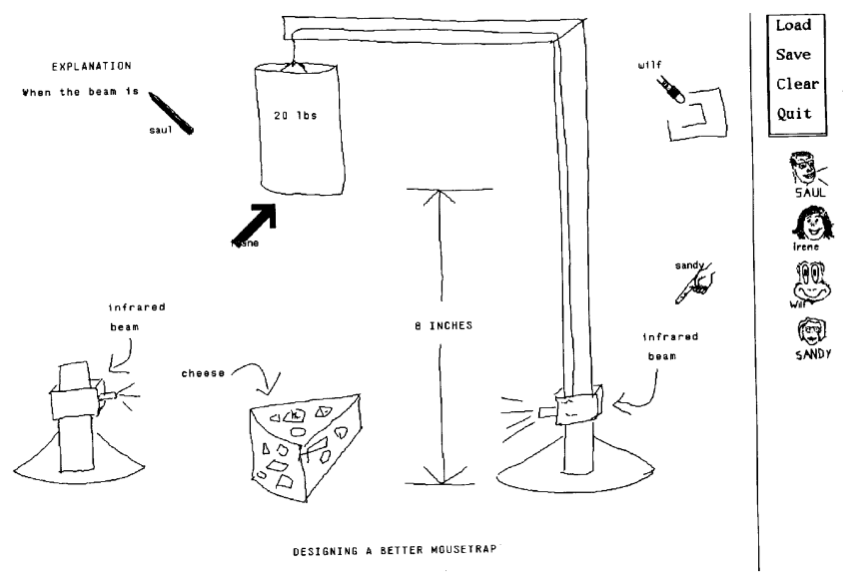
\includegraphics[width=1\linewidth]{gfx/greenbergGroupSketch}}
		\caption[GroupSketch]{Eine typische \emph{GroupSketch} Session mit 4 Teilnehmer. Sie zeigt die Grundfunktionen..}\label{fig:greenbergGroupSketch}
\end{figure}

\subsubsection{XGroupSketch}
\emph{XGroupSketch} verfolgt ein ähnliches Konzept wie \emph{GroupSketch}, unterscheidet sich aber deutlich in einigen wichtigen Punkten. Während \emph{GroupSketch} immer im Vollbildmodus läuft, wird \emph{XGroupSketch} in einem Fenster mit horizontalen und vertikalen Scrollbalken dargestellt. Dadurch handelt es sich streng genommen nicht mehr um einen WYSIWIS-Editor, da nicht mehr gewährleistet werden kann, dass jeder Benutzer zu jedem Zeitpunkt dasselbe sieht. \emph{XGroupSketch} bietet gegenüber \emph{GroupSketch} eine größere Palette an Funktionen. Über mehrere Menüs können die Benutzer unterschiedliche Linienstärken, Farben und Schriften wählen, jedoch bedeutet dies, dass die Applikation weitaus komplizierter in ihrer Bedienung ist, als \emph{GroupSketch}.

\subsubsection{GroupDraw}
Im Gegensatz zu den vorhergehenden zwei rasterbasierten Zeichenprogrammen, ist \emph{GroupDraw} eine objektorientierte Applikation. Da das Design auf den Erfahrungen von \emph{GroupSketch} basiert, wurde das Konzept mit multiplen Cursor und gleichzeitigem Arbeiten beibehalten. Zusätzlich wurden Funktionen wie in strukturierten Zeichen- und Skizzierpaketen (wie z.B. in \emph{Claris MacDraw}) hinzugefügt. Benutzer können nun Zeichenobjekte, wie Rechtecke, Linien, Kreise, Texte, etc. erstellen und diese selektieren und positionieren. Auch bei Groupware wurde das strenge WYSIWIS-Konzept gelockert. Genauso wie in \emph{XGroupSketch} wurde der WYSIWIS Screen durch eine scrollbare Arbeitsfläche ersetzt und bietet den Benutzern zusätzlichen Platz um an privaten Zeichnungen zu arbeiten. \autoref{fig:greenbergGroupDraw} zeigt einen \emph{GroupDraw} Screen mit drei Benutzern, die an einem Design arbeiten. Das kleinere Anmeldefenster listet alle Teilnehmer einer Session auf, deren Standort, Telefonnummer und eine Schnellwahltaste um diese telefonisch zu erreichen.

\medskip Das objektorientierte Konzept und die dadurch gewonnenen Möglichkeiten, bringen eine Reihe an Herausforderungen an das Interface Design bzw. somit auch eine erhebliche Anzahl an möglichen Konflikten mit sich. Bereits die Tatsache, dass Objekte von Benutzern selektiert und verändert werden können, erfordert Maßnahmen zur Tilgung von Konflikten, die auftreten können. So muss überlegt werden, was passieren soll, wenn zwei Benutzer gleichzeitig versuchen, das Objekt zu verändern. Die einfachste Methode ist jene, das Objekt sofort zu sperren wenn ein Benutzer Zugriff erhält. \graffito{Anmerkung zu Scribbler: Wer zuerst kommt, ma(h)lt zuerst.} 
Dazu muss auch eine sinnvolle Art der Visualisierung der Sperre gegenüber anderen Benutzern gefunden werden. Es wäre denkbar, dass das Objekt für jene Benutzer, die gerade keinen Zugriff darauf haben, halbtransparent dargestellt wird. Ebenso muss der Unterschied zwischen dem Selektieren und dem eigentlichen Zugriff auf ein Objekt für die Benutzer verdeutlicht werden. Dazu könnte eine zusätzliche Zeitverzögerung zwischen den beiden Stati helfen. Im vorgestellten Prototyp können Benutzer sofort auf ein Objekt zugreifen und es manipulieren, da das System annimmt, dass keine Konflikte auftreten werden. Falls doch ein Konflikt auftritt und der Zugriff gesperrt wird, schnappt das Objekt zurück zu seiner ursprünglichen Position. In der Praxis erscheint dies jedoch wie ein Flackern, da die Systemreaktion fast unverzüglich stattfindet. 

\medskip Problematisch erweist sich auch der nahtlose Übergang von Aktionen und Funktionen, wie es von Tang \citep{TangJC:1989} empfohlen wird (vgl. \autoref{fig:tangFramework}). Die Tatsache das Benutzer nun aus einer \graffito{Die Auswahl von Objekten aus Paletten oder Menüs, stören den flüssigen Ablauf von Gruppenaktivitäten.}Reihe an Objekttypen auswählen und zusätzlich einen Zeichenmodus auswählen müssen, erschweren Tangs Anforderung. Die Selektion eines Objektes von einer Palette oder einem Menü kann die Kontinuität der Gruppenaktivität stören. Während es in single-user Applikationen grundsätzlich nicht problematisch ist, ein komplexeres Interface zu haben, kann es in multi-user Software eine erhebliche Einschränkung im Workflow der gesamten Gruppe bedeuten. 

\begin{figure}
        {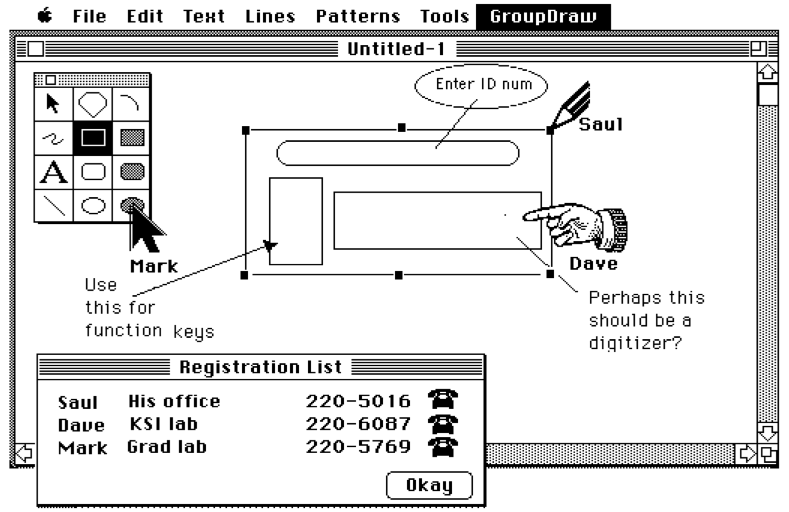
\includegraphics[width=1\linewidth]{gfx/greenbergGroupDraw}}
		\caption[GroupDraw]{Beispiel einer Groupware Session. Sie zeigt die Arbeitsfläche und das Anmeldefenster}\label{fig:greenbergGroupDraw}
\end{figure}

\medskip Ein weiteres Problem sind private Zeichnungen, welche laut Tangs Observationen gute Hilfsmittel darstellen. An ihnen wird oft gearbeitet und der Gruppe erst später präsentiert. \emph{GroupDraw} verfügt über zwei Mechanismen, die dem Schutz der Privatsphäre innerhalb der Gruppe dienen. Einerseits können sich Benutzer durch Scrollen einen eigenen Bereich zum skizzieren suchen und diesen erst nach persönlicher Evaluierung der Zeichnungen den anderen Teilnehmern zeigen. Zum anderen kann jedem Objekt ein >>Verknüpfungstatus<< zugewiesen werden. \citep{Dewan:1991:FUI:108844.108851} 

\subsubsection{GroupKit}
\emph{GroupKit} ist ein Toolkit zur Entwicklung von verteilter Echtzeit-Groupware. Obwohl Applikationen, die mit Hilfe von \emph{GroupKit} entwickelt werden, auch für andere Szenarios als das bloße Zeichnen geeignet sind, waren die Erkenntnisse der zuvor vorgestellten Systeme sehr wichtig für das Design von \emph{GroupKit}.

Die Praxiserfahrungen mit \emph{GroupSketch}, \emph{XGroupSketch} und \emph{GroupDraw} zeigen, dass neben den von Tang definierten Designkriterien \citep{TangJC:1989} noch folgende Faktoren bei der Entwicklung von Groupware Zeichenapplikationen von Bedeutung sind:

\begin{itemize}
	\item
	Die Notwendigkeit einer höheren Telepräsenz
	\item
	Die Möglichkeit nahtloser Übergänge zwischen lokalen, privaten Daten und gemeinsam erstellten Arbeiten zu bieten
	\item
	Berücksichtigung der Anzahl der Benutzer in der Gruppe
\end{itemize}

Die Recherchen \citep{Greenberg:1992p207} haben gezeigt, dass \emph{GroupSketch} und \emph{GroupDraw} während der Zusammenarbeit von räumlich distanzierten Gruppen eine ausreichend hohe Telepräsenz gewährleisten, solange Zeichnen und Skizzieren im Mittelpunkt der Konzeption stehen. Saß die Gruppe im selben Raum, so wandte sich die Aufmerksamkeit vom Computer ab und die Teilnehmer gingen über zu face-to-face Kommunikation, sobald die Skizzen nicht mehr zentrales Thema der Diskussion waren. 

Ferner weisen die Autoren \citep{Greenberg:1992p207} darauf hin, dass es zur Zeit der Untersuchungen (1992) noch zu hohe Barrieren zwischen virtuellen und realen Artefakten gibt. Im Zuge eines Meetings ist es nicht ohne weiteres möglich, echte Artefakte zu digitalisieren und mit anderen zu teilen.

Letztlich ist die Anzahl der Benutzer ein kritischer Faktor für die Art und Weise, wie eine gemeinsame Zeichenfläche genutzt wird. Die vorgestellten Systeme \emph{GroupSketch} und \emph{GroupDraw} funktionieren gut im Einsatz mit Gruppen die aus 2-4 Personen bestehen. Sehr häufig arbeiten aber weitaus mehr Menschen zusammen und es bleibt die Frage im Raum, ob die Systeme dementsprechend skalieren. Ein Test mit acht Teilnehmern hat bereits einige Problemstellen entlarvt. Das Konzept der multiplen Cursor kann sehr schnell dazu führen, dass der Bildschirm überfüllt wirkt und die vielen Bewegungen mögen etwas irritierend sein. Um diesem Phänomen entgegen zu wirken, verkleinern sich die Cursor entsprechend ihrer Anzahl. Wenn Benutzer bestimmte Aktionen durchführen, vergrößert sich der jeweilige Cursor während dessen wieder auf normale Größe, damit Interaktionen gut erkennbar bleiben. 

\subsection{Screencrayons}
Anders als bei den bis jetzt vorgestellten Systemen, die sich mit kollaborativen Zeichnen befassten, konzentrierten sich Olsen, Jr et al. mit \emph{ScreenCrayons} 2004 - über ein Jahrzehnt später - auf den praktischen Aspekt von Zeichentools, nämlich auf barrierefreies Zeichnen bzw. Annotieren über die Grenzen eines Programmfensters hinaus.
Der Stein der ihr Projekt ins Rollen brachte, war eine Studie von Adler et al. \citep{Adler:1998}, in der gezeigt wurde, dass Probanden, beim Arbeiten an Dokumenten, 70\% mit Lesen verbringen und einen maßgeblichen Teil dieser Zeit mit Schreiben vermischen. Beim Erstellen und Bearbeiten von Dokumenten wird laut Studie zwar nur 18\% während dem Lesen geschrieben, jedoch benötigt das Anmerken und Schreiben von Notizen davon 48\% der Zeit. Schilit beschreibt dies als >>aktives Lesen<< \citep{Schilit:1998}, bei dem die Person die gelesenen Informationen \emph{verbessert, aussortiert, hervorhebt, zusammenfasst und organisiert}. Hier haken Olsen, Jr et al. \citep{Olsen:2004} ein und versuchen eine möglichst vielseitig einsetzbare computerunterstützte Software zu entwickeln, die diese Aktivität unterstützt.

\medskip Aber warum softwarebasiert? Die grundlegende Metapher für moderne Computerworkstations ist Papier. Seit den Anfängen des \emph{Xerox Stars\footnote{Der Xerox Star (Xerox 8010) wurde 1981 von der Xerox Systems Development Division entwickelt. Er war der erste kommerzielle PC mit einer anwenderfreundlichen grafischen Benutzeroberfläche, bestehend aus einen per Maus bedienbaren Desktop mit Menüs und Fenstern.}}, wurden Programmfenster so modelliert, dass sie Seiten an Papier ähneln. Die meist benutzten Textverarbeitungs-, Zeichen- und Tabellenkalkulationsprogramme benutzen diese Metapher. 
In der Zeit vor Computern gab es zwar Schreibmaschinen zum Verfassen von Dokumenten, jedoch waren diese nicht besonders einfach zum handhaben, wenn es darum ging Fehler auszubessern. Papierdokumente abzuändern oder in Umlauf zu bringen wurde dadurch ebenfalls erschwert. Das einzige was einfach war, war auf den Dokumenten Markierungen und Anmerkungen anzufertigen, da dies handschriftlich geschah.
Durch diese Ungleichheit wurde der Fokus der meisten Bürosoftwaretools auf das >>schwere<< Erstellen und Veröffentlichen bzw. Verbreiten von Dokumenten gesetzt und das Annotieren außen vor gelassen. Aber gerade in heutiger Zeit, wo der Speicher immer billiger wird, über das Internet kommuniziert wird und der Computeraufschwung bzw. die Einführung von Standardformaten wie \emph{PDF\footnote{Portable Document Format}} oder \emph{HTML\footnote{Hypertext Markup Language}} eine Verlagerung der Benutzung von Dokumenten hervorruft, ist der Großteil der Leseaktivität digital geworden. Ein digitales Annotierungstool ist somit eine naheliegende Erweiterung.

\medskip Anhand eines ausführlichen Szenarios überlegten sich Olsen, Jr et al. im Vorfeld folgende Punkte, die das Anfertigen von Notizen mit sich bringt:

\begin{enumerate}
	\item Notizen entstehen spontan während der Arbeit und müssen nicht zwangsweise mit der derzeitigen Aufgabe zusammenhängen.
	\item Notizen entstehen im Zusammenhang mit vielen Applikationen. Im Szenario wurden z.B. ein Email-Client, ein Textverarbeitungsprogramm, ein Tabellenkalkulationsprogramm, ein Webbrowser, ein PDF Reader und eine eigens geschaffene Spezialsoftware verwendet.
	\item Notizen sind häufig Zusammenfassungen oder hervorgehobene Auszüge vom Gelesenen. Sie dienen dazu die Aufmerksamkeit an sich zu ziehen, damit man in Zukunft nicht erneut das gesamte Dokument lesen muss.
	\item Notizen sind oft der Ausgangspunkt für späteres Schreiben (z.B. für eine Zusammenfassung).
	\item Notizen können verschiedene Informationsquellen miteinander verknüpfen, in denen Zusammenhänge gefunden wurden. Z.B. kann ein Zitat mit einem anderen Artikelabschnitt verknüpft werden.
\end{enumerate}

Die meisten Annotierungsysteme unterstützen lediglich das Erstellen von Anmerkungen auf spezifischen Artefakt- bzw. Dokumententypen. Das Erlernen von solchen Notizsystemen für jede einzelne Anwendung ist dabei nicht nur unangenehm sondern auch mühsam. Das Ziel von \emph{ScreenCrayons} ist es, eine einfache und universelle Software zur Verfügung zu stellen, die unabhängig von Programmimplementierungen oder Dateitypen arbeitet und alle oben genannten Bedürfnisse erfüllt, ohne andere Arbeiten damit zu beeinflussen. Sie soll über die gesamte Arbeit des Benutzers wirken.

\medskip Eine universelle Annotierungsmöglichkeit zu schaffen, ist zwangsweise eine Herausforderung. In Hinblick auf die Softwarearchitektur wäre der einfachste Ansatz für alle Artefakte, an denen Notizen vorgenommen wurden, ein >>Special Purpose Model\footnote{Model bzw. dt. Modell, ist ein Bestandteil des 1979 ins Leben gerufene MVC (Model-View-Controller) Softwarearchitekturmusters. Ziel des Musters ist eine spätere Änderung oder Erweiterung zu erleichtern und eine Wiederverwendbarkeit der einzelnen Komponenten zu ermöglichen. Die Modellkomponente enthält die darzustellenden Daten und ist von Präsentation und Steuerung unabhängig.}<< zu erstellen. Alle Notizen, die in den einzelnen Programmen erstellt werden, müssten in dieses Modell >>übersetzt<< werden. 

Der Vorteil dieses Ansatzes wäre, dass die Notizen in die Modellrepräsentation eingebettet werden können und somit eine Vielzahl an Visualisierungen (der Notizen in Verbindung mit dem zugehörigen Inhalt) designed und implementiert werden können. Der Nachteil den das Artefaktmodelldesign mit sich bringen würde wäre, dass dokumentorientierte, oder digital-ink Ansätze einen Übersetzer erfordern. Falls für eine Applikation kein Übersetzer existiert, gibt es auch keine Annotierungsmöglichkeit.

\medskip Die zweite Möglichkeit wäre ein eigenes Protokoll zu entwickeln, das alle Applikationen verwenden. So ein Protokoll würde Signale wie >>hier ist ein Digital-Ink Strich, liefere mir eine Notizreferenz<<, >>hier ist eine Notizreferenz, zeig sie in der Applikation<< und >>hier ist eine Notizreferenz, liefere mir ihre \emph{Bounding Box\footnote{Eine Bounding Box oder auch minimal umgebendes Rechteck, ist das kleinstmögliche achsenparallele Rechteck, das ein oder mehrere geometrische Objekt(e) umgibt.}} am Bildschirm<< umfassen. Zusätzlich würde es allen Applikationen, die das Protokoll verwenden, erlauben Notizen hinzuzufügen. Die große Aufgabe wäre alle interessanten Applikationen mit dem Protokoll auszustatten.

\medskip Mit \emph{ScreenCrayons} entschieden sich Olsen, Jr et al. zu einem dritten Ansatz, der hingegen vollkommen im Bildraum arbeitet. Dadurch müssen zwar alle Applikationen ihre Informationen als Bilder bereitstellen, jedoch ist dies nicht weiters problematisch, da alle größeren fensterbasierenden (Betrieb-)Systeme die Möglichkeit bieten, Abbildungen des Bildschirms (sog. \emph{Screenshots}) zu erstellen. \graffito{Ein universelles Annotierungsprogramm benötigt ein universelles Medium um Notizen auf beliebigen Content zu erstellen.} Somit besteht ein universelles Medium um Notizen auf aller Art an Information zu erstellen, ohne direkt mit der Applikation >>kooperieren<< zu müssen. Das ist ein wichtiger Schritt um Annotierungen universell einsetzbar zu machen. Der Nachteil dieses Ansatzes ist jedoch, dass die Notizen - ohne Zugang zu einem Modell - keine strukturellen Vorteile mit sich bringen und sich somit total unintelligent verhalten. \emph{ScreenCrayons} versucht daher \graffito{Scrolling befördert einen Teil des Annotierungskontextes aus dem Blickfeld.} eigenständig, aus dem Bildmaterial eine simple Struktur zu entnehmen. Ein Nachteil, dem \emph{ScreenCrayons} jedoch nicht entgegenwirken kann, entsteht z.B. durch Scrolling\footnote{Scrolling: dt. Bildlauf} eines Dokuments, da ein Teil des nicht sichtbaren Kontextes verloren geht.

\medskip Olsen, Jr et al. fassen somit die für sie wichtigsten Anforderungen an ein Annotierungstool wie folgt zusammen:

\begin{enumerate}
	\item Notizen müssen im Kontext, passend zu der jeweiligen Arbeit, erstellt werden - nicht in einem seperaten Programm.
	\item Das Erstellen von Notizen muss eine leicht anwendbare Tätigkeit sein, die keinen großen Aufwand mit sich bringt.
	\item Eine Notiz muss den visuellen Kontext, in dem sie erstellt wurde, erhalten.
	\item Die entstehenden Notizen müssen in kompakter, zusammengefasster Form verfügbar gemacht werden, damit sie nachträglich leicht durchstöbert und geändert werden können.
\end{enumerate}

In \emph{ScreenCrayons} besteht eine Notiz aus einem Namen, einen Screenshot, dem Gezeichneten und kein oder mehreren Kommentaren. Um etwas zu annotieren, muss der Benutzer also 
\begin{inparaenum}[\itshape 1\upshape)]
\item kennzeichnen an welchem digitalem Artefakt eine Notiz angebracht werden soll,
\item dem Artefakt ein Thema zuweisen, um die Notiz zu kategorisieren und
\item optional Kommentare hinzufügen, um zu zeigen was an der Notiz wichtig ist.
\end{inparaenum}

\medskip Die zentralen Instrumente in \emph{ScreenCrayons} sind, wie der Name schon verrät, die sog. Crayons. Sie sind Digital-Ink Spender, welche in einer >>Crayon Box<< aufbewahrt werden. Findet der Benutzer eine interessante Stelle, die er gerne kommentieren möchte, schaltet er in den >>Crayon Modus<<, schnappt sich einen Crayon aus der Box und benutzt ihn um Stellen am Screen hervorzuheben. Diese >>auf dem Bildschirm kritzeln<< Metapher ist einfach zu erlernen und \graffito{Eine >>auf dem Bildschirm kritzeln<< Metapher ist einfach und universell einsetzbar.}komplett unabhängig von anderen Applikationen.
Das Erfassen von Notizen geschieht mit Hilfe von Screenshots. Dabei reicht es aber nicht die Screenshots einfach abzuspeichern, da die Ergebnisse unbrauchbar groß wären. Statt dessen können die Benutzer von \emph{ScreenCrayons} interessante Stellen annotieren und das Programm errechnet aus dieser Information den Bereich, der erfasst werden soll. Erkannt werden Kreise, die Text umgeben und Striche, die Text entweder unterstreichen, durchstreichen oder seitlich markieren. Die errechnete Boundingbox zieht sich bis an die Textgrenzen, wodurch der Kontext erhalten bleibt. (siehe \autoref{fig:olsenRegionFinding}) 

\medskip Beim Schalten in den Crayon Modus wird zuerst ein Screenshot angefertigt und über den gesamten Screen bzw. alle Fenster gelegt. Der Benutzer sieht zwar keine Änderung, jedoch sind dadurch alle Applikationen scheinbar stillgelegt. Mauseingaben werden zu Zeichnungen auf dem Bildschirm, anstatt zu den jeweiligen Applikationen weitergeleitet zu werden. Um dem Benutzer zu zeigen in welchen Modus er sich befindet, \graffito{Modi sollten visuell, z.B. durch farbliches Einrahmen eines Fensters, erkennbar gemacht werden.} wird das aktive Fenster mit einem halbtransparenten Rahmen versehen, in der selben Farbe wie der ausgewählte Crayon. Alle Hintergrundapplikationen hingegen werden mit einer hellen Farbe überblendet um die Blicke davon abzulenken. Die >>Crayon Box<< erscheint ebenfalls am Screen und bietet verschiedene Optionen, wie die Auswahl anderer Crayons, das Speichern von Notizen, das Abbrechen vom Notizerstellvorgang oder das Ändern von Crayons. (siehe \autoref{fig:olsenHighlighting})

\medskip Die gesammelten Annotationen, bestehend aus Screenshots, den Highlightings und Kommentaren, können für den Benutzer auf verschiedene Arten visualisiert werden. \autoref{fig:olsenRepresentation} zeigt die drei verschiedenen Annotationsrepräsentationen mit ihren unterschiedlichen Kontextdetailgraden.

\medskip Das manuelle Umschalten vom Benutzer \graffito{Manuelles Umschalten von Modi ist mühsam.} zum >>Crayon Modus<< ist zwar mühsam aber notwendig. Ohne Kontrolle auf die laufenden Applikationen gibt es keinen anderen Weg um zwischen den Annotierungseingaben und den Applikationseingaben zu unterscheiden. Jede Annotierungseingabe via Stift oder Maus könnte genauso gut als Eingabe der darunterliegenden Applikation aufgefasst werden. Das Überlagern vom gesamten Bildschirm mit dem Annotierungsscreenshot bewahrt den Kontext jeder Applikation und zeigt, dass Eingaben nun Annotierungen sind - keine Applikationsoperationen.

\bigskip \emph{Anmerkung: \graffito{\(\clubsuit\)}Die Problematik der Modiumschaltung wird im Kapitel \nameref{ch:DesignVSComputer} unter dem Abschnitt \nameref{sec:ModusProblem} näher beschrieben.}

\begin{figure}
        {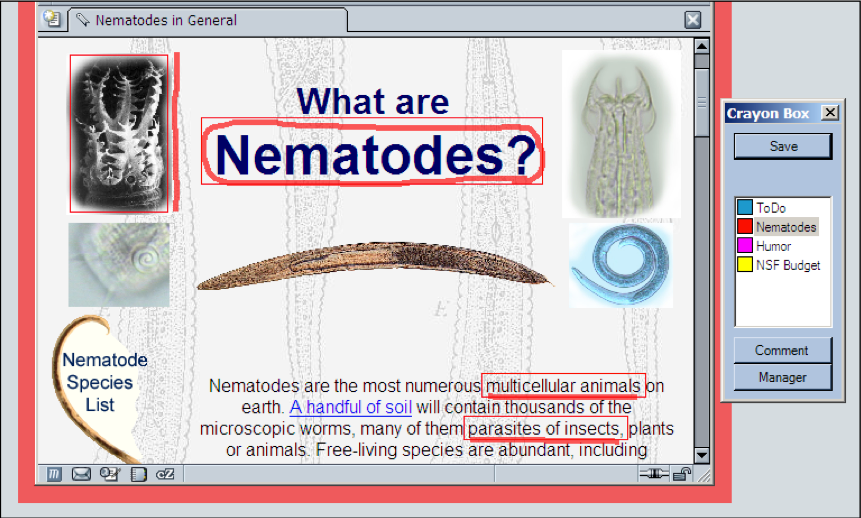
\includegraphics[width=\linewidth]{gfx/olsenHighlighting}}
		\caption[Crayon Highlighting.]{Der Zeichenmodus. Charakterisiert durch die Hervorhebung des aktuellen Fensters mit einem Rahmen in der aktuellen Crayonfarbe und der Crayon Box. Alle Hintergrundapplikationen werden überblendet.}\label{fig:olsenHighlighting}
\end{figure}

\begin{figure}
        {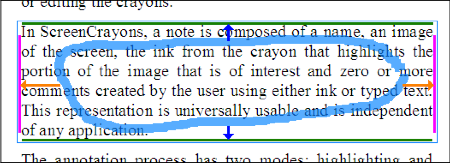
\includegraphics[width=\linewidth]{gfx/olsenRegionFinding}}
		\caption[Finding Regions for Circles/Scribbles.]{Visualisierung der Bereichsberechnung. Kreise und Gekritzel bilden die Grundlage zur Berechnung der Boundingbox. Der Kontext bleibt bewahrt.}\label{fig:olsenRegionFinding}
\end{figure}

\begin{figure}
        \myfloatalign

 			\begin{tabular}{ l r }
				%\multirow{2}{*} {
				\raisebox{-18.4mm}{
				\subfloat[Alle Highlights und Kommen-tare.] 
	        		{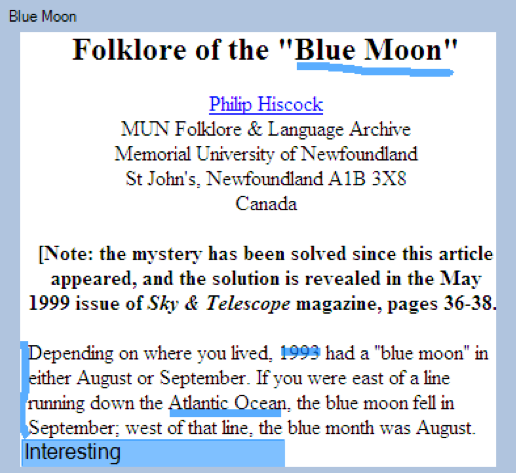
\includegraphics[width=.445\linewidth]{gfx/olsenRepresentation1}} } &
				
				\begin{tabular}{ l }
					\subfloat[Alle interessanten Bereiche, inkl. Kommentare.]
		        		{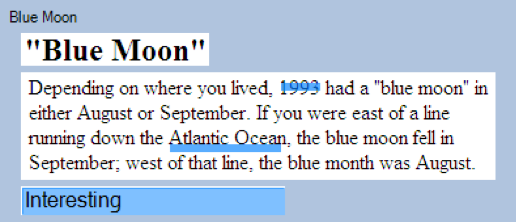
\includegraphics[width=.45\linewidth]{gfx/olsenRepresentation2}} \\
					\subfloat[Direkt markierte Texte und Kommentare.]
						{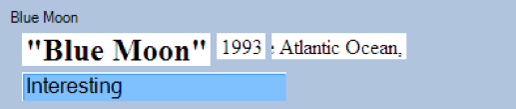
\includegraphics[width=.45\linewidth]{gfx/olsenRepresentation3}} \\
				\end{tabular}
			\end{tabular}
        	
        \caption[Drei verschiedene Repräsentationen eines Annotationsbeispiels.]{Drei verschiedene Repräsentationen eines Annotationsbeispiels. (a) zeigt alle Annotierungen im original Dokument mit zusätzlichem Kommentar. (b) zeigt die Annotierungen reduziert auf die interessanten Bereiche und zusätzlichem Kommentar und (c) zeigt die davon direkt angezeichneten Texte und den Kommentar.}\label{fig:olsenRepresentation}
\end{figure}

\subsection{Ein Tablet unterstütztes Meetingtool}
2007 entwickelnden Bastéa-Forte und Yen ein kollaboratives Skizziertool, dass mehreren Benutzern erlaubt gleichzeitig auf einer gemeinsamen Arbeitsfläche zu arbeiten. Ihr System umfasst Tablet PCs mit integrierten Screens für jeden Teilnehmer und ein digitales Whiteboard für die Gruppe. Auf den Geräten wird eine vernetzte Skizzierapplikation ausgeführt, welches jedem Gruppenteilnehmer erlaubt die gemeinsame Skizzierfläche zu sehen und auf ihr zu zeichnen (siehe \autoref{fig:basteaSketchingSystemB}). Sie sind der Auffassung, dass die Zugangsgleichstellung vom Betrachten und Zeichnen die Hemmschwelle zum Mitzeichnen senkt und dass das Arbeiten im selben Raum die Kollaboration fördert. 

\begin{figure}
        \myfloatalign
        \subfloat[Skizzierfläche]
        {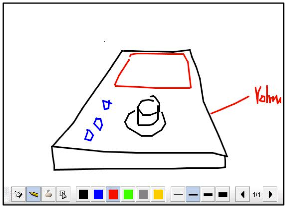
\includegraphics[width=.6\linewidth]{gfx/basteaSketchingSystemA}} \quad
        \subfloat[Setting]
        {\label{fig:basteaSketchingSystem}%
         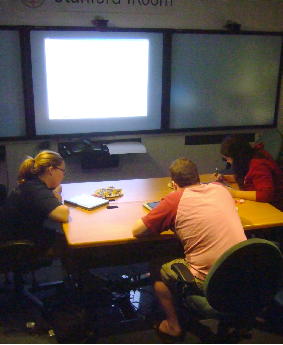
\includegraphics[width=.35\linewidth]{gfx/basteaSketchingSystemB}} \\
        \caption[Das kollaborative Skizziersystem.]{Das kollaborative Skizziersystem ermöglicht gleichzeitige Sicht und Eingaben auf eine gemeinsam genutzte Skizzierfläche (a) durch vernetzte Tablet PCs und einem digitalen Whiteboard. (b) }\label{fig:basteaSketchingSystemB}
\end{figure}

\medskip Das kollaborative Skizziersystem ist ein Zeichenprogramm welches in Java 5 realisiert wurde und auf den Tablet PCs bzw. dem digitalen Whiteboard läuft. Die Skizzierfläche wird auf allen Geräten >>gespiegelt<<, sodass jede auf dem Tablet kreierte Zeichnung sofort auf den anderen Tablets und dem Whiteboard sichtbar wird. Dadurch wird interaktives kollaboratives Skizzieren ermöglicht. So kann beispielsweise beim Designen eines Fernsehgerätes, ein Teilnehmer die Grundrisse zeichnen und ein weiterer gleichzeitig beginnen die Knöpfe hinzuzufügen. Alle Benutzer können mit Leichtigkeit gleichzeitig Skizzen sehen und neue hinzufügen. 

\medskip Das Programm bietet Tools zum Freihandzeichnen und Löschen verschiedener Linienfarben \& -stärken und eine Freiformselektion um Striche innerhalb einer Seite zu bewegen. Jeder Cursor ist mit dem Namen des jeweiligen Teilnehmers gekennzeichnet und erscheint am Whiteboard beim Zeichnen, Selektieren oder Löschen. Den Benutzern steht auch ein \emph{Gesture Tool} zu Verfügung, das es ihnen erlaubt bestimmte Regionen auf der Arbeitsfläche hervorzuheben. Die Applikation unterstützt mehrere Seiten. Die Navigation zwischen den Seiten betrifft alle Displays und hält die Gruppe >>auf der selben Seite<<.

\medskip Bastéa-Forte und Yen gingen davon aus, dass das vorgestellte Setting die Hemmschwelle zum Mitzeichnen in Gruppenmeetings verringern wird, die Gesamtanzahl an Skizzen steigen wird und die Teilnehmer gleich stark mitarbeiten werden. Um diese These zu überprüfen, führten sie Untersuchungen mit Studentengruppen aus den Bereichen HCI und Maschinenbau der Universität in Stanford durch. Fünf Gruppen zu je drei Studenten wurden mit Tablet PCs und einem digitalen Whiteboard ausgestattet, die miteinander vernetzt waren und eine gemeinsame Zeichenfläche zeigten. Im >>Kontrollzustand<< waren die Geräte von einander isoliert und zeigten von einander unabhängige Zeichenflächen, um Tools aus konventionellen Gruppenmeetings nachzuahmen. Im >>Experimentalzustand<< waren die Geräte miteinander vernetzt. \autoref{fig:basteaConditionExperimental} zeigt die beiden Zustände gegenübergestellt.

\medskip Am Anfang der Untersuchung, wurden den Teilnehmern die digitalen Tools und das Programm erklärt. Nach einer 10 minutigen Eingewöhnungsphase wurde der Gruppe 30 Minuten Zeit gegeben um ein Design für eine Multifunktionsfernbedienung (für einen Herd, einen Backofen und eine Stereoanlage) zu erarbeiten. Anschließend hatten sie eine Minute Zeit um ihr finales Design zu präsentieren. Die Aufgabe war eine vereinfachte Version derer, wie sie in \citep{Tang1991143} an Kleingruppen gestellt wurde. Nachträglich mussten die Teilnehmer einen Fragebogen mit je 20 Likert-Skala\footnote{Die Likert-Skala ist ein Skalierungsverfahren zur Messung persönlicher Einstellungen, die durch sog. \emph{Items} abgefragt werden. Die Antwortmöglichkeiten für ein Item, bilden den Grad der Zustimmung der befragten Person. Z.B.: Trifft zu - Trifft eher zu - Weder noch - Trifft eher nicht zu - Trifft nicht zu. Verwendung finden Likert-Skalen in Fragebogenerhebungen, insbesondere in der empirischen Sozial-, Markt- und Wahlforschung und der Psychologie.} Fragen und sechs offenen Fragen, über Gruppenteilnahme, Gruppendynamik, Brainstormingstrategien und Brauchbarkeit des Systems in Bezug auf Kommunikation und Aufgabenlösung, beantworten. Zusätzlich gab es eine Nachbesprechung, in der die Teilnehmer über ihre Erfahrungen mit dem System befragt wurden. Die Server Applikation sammelte während der gesamten Zeit über Daten durch Aufzeichnen der Zeichen- und Zeigeeingaben in einem Logfile.

\begin{figure}
        \myfloatalign
        \subfloat[Kontrollzustand]
        {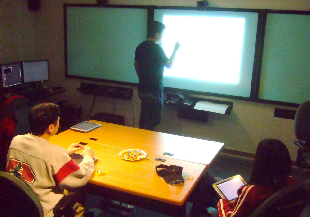
\includegraphics[width=.48\linewidth]{gfx/basteaConditionControl}} \quad
        \subfloat[Experimentalzustand]
        {\label{fig:basteaConditionControl}%
         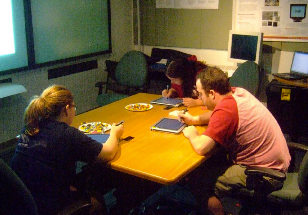
\includegraphics[width=.48\linewidth]{gfx/basteaConditionExperimental}} \\
        \caption[Die unterschiedlichen Arbeitszustände im Vergleich.]{Die unterschiedlichen Arbeitszustände im Vergleich. Im Kontrollzustand arbeiten die Teilnehmer an einer Brainstormingaufgabe mit von einander unabhängigen Geräten - Tablet PCs und digitalem Whiteboard (a) - und im Experimentalzustand mit vernetzten Geräten (b)}\label{fig:basteaConditionExperimental}
\end{figure}

\begin{figure}
        \myfloatalign
        \subfloat[Mittlere Standardabweichung vom prozentuellen Skizzierbeitrag jedes Teilnehmers]
        {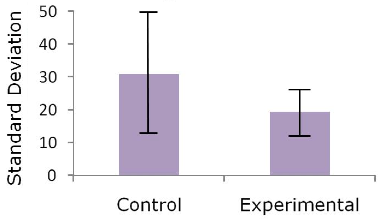
\includegraphics[width=.48\linewidth]{gfx/basteaEvaluationDeviation}} \quad
        \subfloat[Mittelwert der gesamten Skizziereingaben aller Gruppen]
        {\label{fig:basteaEvaluationSketchingInput}%
         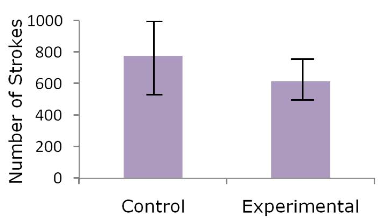
\includegraphics[width=.48\linewidth]{gfx/basteaEvaluationSketchingInput}} \\
        \caption[Logfile Analyse]{Statistische Analyse des Logfiles. Sie zeigt das schlechte untereinander aufgeteilte Skizzierverhalten (a) und die dafür größere Anzahl an Gesamtskizzen (b) im Kontrollzustand im Gegensatz zum Experimentalzustand.}\label{fig:basteaEvaluationDeviation}
\end{figure}

\begin{figure}
        {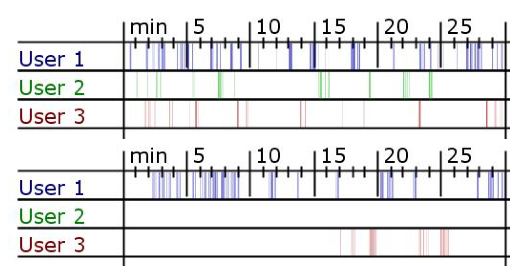
\includegraphics[width=0.9\linewidth]{gfx/basteaEvaluationStrokes}}
		\caption[Repräsentationen der Strichstatistik.]{Darstellung der Strichhäufigkeit zweier Gruppen. Die Ergebnisse der Experimentalgruppe (oben) zeigen deren Interaktivität beim Skizzieren. Im Gegensatz die Kontrollgruppe (unten), mit nur einzelnen Wechsel zwischen den Teilnehmern.}\label{fig:basteaEvaluationStrokes}
\end{figure}

\medskip Die gesammelten Zeichendaten deuten darauf hin, dass die Skizzierverteilung im Experimentalzustand innerhalb der Gruppe eher ausgeglichen ist. Die Standardabweichung des Mittelwerts, über den prozentuellen Anteil an gezeichneten Strichen pro Benutzer, war ebenso wie angenommen kleiner als im Kontrollzustand (p = 0.17, siehe \autoref{fig:basteaEvaluationDeviation})
Der relative Skizzierbeitrag eines Benutzers ergibt sich aus dem Prozentsatz an Strichen, die ein Benutzer einer Gruppe gezeichnet hat. Dessen Standardabweichung zeigt die Schwankungen innerhalb der Gruppe. Im Gegensatz zu der anfänglichen Annahme, zeigen die Zeichendaten, dass der durchschnittliche Zeicheninput der Kontrollgruppen größer als der der Experimentalgruppen ist (p = 0.21).
Die meisten Kontrollgruppen folgtem einem typischen Meetingablauf, gezeichnet durch einen selbsterkorenen Schreiber am Whiteboard und den sitzenden Gruppenteilnehmern, die gelegentlich die Tablet PCs für private Skizzen nutzten und diese manchmal später der Gruppe zeigten. Im Gegensatz dazu näherte sich die Experimentalgruppe kaum dem Whiteboard. Durchschnittlich 57\% aller gezeichneten Striche der Kontrollgruppen waren auf dem Whiteboard zu finden - in der Experimentalgruppe lediglich 4.4\% (p = 0.01). Die Antworten der Fragebögen bzw. die informellen Interviews der Nachbesprechung weisen darauf hin, dass das digitale Whiteboard im Experimentalzustand hauptsächlich zum Betrachten der Zeichnungen benutzt wurde und den Fokus der Gruppe erhielt. Trotz der gespiegelten Sicht auf die Tablet PCs, meinten Experimentalteilnehmer, dass das Whiteboard \graffito{Ein gemeinsam genutztes Whiteboard ist ein wichtiger Bestandteil kollaborativen Arbeitens.} wichtig war um zu sehen was jeder arbeitet und alle Zusammenhänge zu erkennen. Weiters mochten sie die Tatsache, nicht aufstehen zu müssen um das Whiteboard zu benutzen. Eine Gruppe sagte sogar, dass durch die einzelnen Geräte das Whiteboard scheinbar mehr Macht erhielt, was sie daran hinderte es direkt zu benutzen, wie sie es vielleicht ohne den Geräten getan hätten.

\medskip Teilnehmer merkten weiters an, dass das System im Gegensatz zu traditionellen Tools von Anfang an klar stellt, wer welche Zeichnung beisteuert. Zusätzlich nehmen sie im Experimentalsystem bewusster wahr, wieviel jede Person zeichnet und halten sich deswegen sogar in manchen Fällen mit dem Zeichnen zurück. Eine Gruppe klammerte sich an diesen Aspekt und entschied Farben zur Kennzeichnung der Skizzen zu verwenden. Darüber hinaus sagten einige Teilnehmer, dass sie unsicherer über die Qualität der Ideen sind, die sie auf das Whiteboard legten. So fühlen sie z.B. eine >>bedingungslose Verantwortung<< für ihre Zeichnungen, mit der Angst keine >>echten Beiträge<< zu leisten. Einige Teilnehmer berichteten, dass sie über Ideen länger nachdachten, um sie ausgereifter der Gruppe mittels Skizzen zu präsentieren.
Das ausgeprägtere Bewusstsein über die Qualität und Quantität der Beiträge, erklärt möglicherweise warum weniger Zeichnungen im Experimentalzustand gemacht wurden. Die geringere Beitragsrate widerspricht jedoch dem >>go for quantity<< Leitsatz von Brainstormings. Bastéa-Forte und Yen vermuten, dass dieses Bewusstsein aufgrund einer expliziten Skizzenidentifikation entsteht oder durch die Tatsache, dass Skizzen mehr ausdrücken als Worte. 

\medskip Im Experimentalzustand wurde öfter interaktives kollaboratives Zeichnen beobachtet (siehe \autoref{fig:basteaEvaluationStrokes}). Gruppenmitglieder tendierten dazu an andere Zeichnungen anzuknüpfen, indem sie Notizen zu existierenden Skizzen hinzuschrieben oder eine alternative Idee daneben aufzeichneten. In einer Gruppe bildeten alle drei Teilnehmer Listen von Ideen, in denen jeder Punkte hinzufügte. In anderen Gruppen wiederum, wurde ein Schreiber ernannt.
Den Teilnehmern fiel auf, dass ihnen die Möglichkeit, während ein Kollege spricht oder zeichnet gleichzeitig skizzieren zu können, sehr gefällt. Bei konventionellen Tools würde das Nähern einer weiteren Person zum Whiteboard, die Aufmerksamkeit der Gruppe an sich ziehen. Das vorgestellte System erlaubt hingegen den Teilnehmern Ideen ohne Unterbrechung >>zu Papier zu bringen<<. 
Eine genannte Konsequenz des Systems, war die Reduktion der Face-To-Face Kommunikation. Die Teilnehmer waren zu sehr beschäftigt auf die Skizzen ihres Tablet PCs zu achten, dass sie sich untereinander weniger ansahen. Andererseits besteht das Problem auch bei konventionellen Whiteboardpraktiken, da die Gruppenmitglieder neigen zum Whiteboard zu schauen, anstatt zu den Kollegen.
Trotz dem unbegrenzten virtuellen Zeichenplatz, hat das System nur einen limitierten Platz am Tabletdisplay. Teilnehmer erwähnten, dass die Handhabung manchmal schwer war, da sie öfters mehrere Skizzen gleichzeitig im Blick haben wollten.

\medskip Alles in allem zeigte die Studie die Auswirkungen von gemeinsamen Zeichnen auf Brainstormings. Der Zugriff auf eine gemeinsam genutzte Skizzierfläche mittels vernetzter Tablet PCs und einem digitalen Whiteboard, schafft eine gleichmäßige Zeichenbeteiligung der einzelnen Gruppenmitglieder, da die eigenen Geräte die Beteiligungshemmschwelle heruntersetzt. Völlig unerwartet zeigen die Ergebnisse aber auch, dass das System die Gesamtanzahl an Skizzen beeinflusst. Es werden zwar weniger Skizzen gezeichnet, jedoch wird das Bewusstsein für die Anzahl an Beiträgen pro Teilnehmer gestärkt und somit die Qualität der Beiträge angehoben.

\medskip Als nächsten Schritt sehen Bastéa-Forte und Yen ein Hybridsystem, in dem eine private Zeichenfläche zum bestehenden System, mit der geteilten öffentlichen Zeichenfläche, hinzugefügt wird. Sie glauben, dass eine Fläche zum privaten \graffito{Eine zusätzliche private Zeichenfläche könnte mögliche Zeichenhemmungen nehmen.} Entwickeln von Ideen - mit der öffentlichen Fläche in Sichtweite - helfen würde, den Hemmungen (von denen ein paar Teilnehmer berichteten) entgegenzuwirken. Durch Beisammenhalten der privaten und öffentlichen Zeichenfläche, können Benutzer Skizzen anfertigen ohne den Anschluss an die Gruppendiskussion zu verlieren und Ideen einfach zwischen den beiden Flächen übertragen.
Weiters sind sie daran interessiert die Vorteile des digitalen Whiteboards, beispielsweise durch das Erhöhen der Anzahl an sichtbaren Skizzen oder durch dessen Einsatz als zentralen Blickfänger, auszureizen. Eine Möglichkeit dies zu bewerkstelligen wäre, das Whiteboard zu benutzen, um mehrere Seiten gleichzeitig anzuzeigen bzw. über größere Flächen navigieren zu können.

\subsection{Team Storm}
\emph{Team Storm} \citep{Hailpern:2007p113} ist ein Groupware System, das die Möglichkeit bietet, parallel an mehreren Ideen zu arbeiten. Es kommt bei Meetings in frühen Konzeptionsphasen zum Einsatz und fördert Kreativität innerhalb der Gruppe. Es konzentriert sich auf das Skizzieren von Ideen und bietet private und gemeinsame Arbeitsflächen, auf denen die Designer arbeiten können.

Das System besteht aus drei Hauptkomponenten: den sogenannten Canvases und den privaten sowie gemeinsamen Arbeitsbereichen. Eine Skizze, bzw. ein Design repräsentiert einen Canvas. Die Benutzer können eine beliebige Anzahl an Skizzen erstellen, dabei verwenden sie entweder Tablet-PCs oder andere stiftbasierte Eingabegeräte. 

Zeichnungen werden durch Icons dargestellt, die beliebig auf der privaten Arbeitsfläche (\autoref{fig:teamStorm}, unteres Fenster) positioniert und skaliert werden können. Diese Darstellung bietet deutliche Vorteile: Designer können Relevanz und Fortschritt selbst definieren und die Skizzen dementsprechend anordnen bzw. skalieren. Durch diese Freiheit können ebenso semantisch verknüpfte Zeichnungen zu Gruppen zusammen geordnet werden. Der Nachteil dieser Methode ist der hohe Platzbedarf auf dem Monitor oder dem Tablet-PC.

Auf der gemeinsamen Arbeitsfläche (\autoref{fig:teamStorm}, oberes Fenster), können Designer ihre Canvases mit den anderen Sitzungsteilnehmern teilen, diskutieren, überarbeiten und organisieren. Dieser Bereich, der für jeden vollständig sichtbar ist, bietet allen Benutzern die selben Möglichkeiten wie der private Arbeitsbereich. \autoref{fig:teamStorm} zeigt im oberen Programmfenster eine exemplarische Anordnung mehrerer Skizzen, die von verschiedenen Designern angefertigt und mit den anderen geteilt wurden. \\

\begin{figure}[bth]
	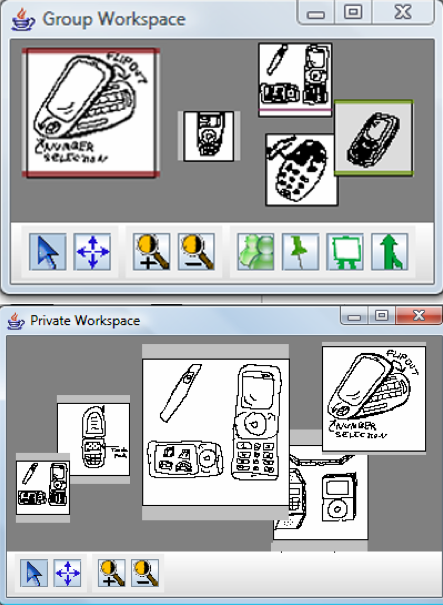
\includegraphics[width=\linewidth]{gfx/teamStormPrivateWorkspace.png}
	\caption{Gemeinsame und private Arbeitsbereiche in \emph{Team Storm}. Designer können ihre Skizzen räumlich anordnen und die Größe anpassen.}
	\label{fig:teamStorm}
\end{figure}

Während ein Designer eine Skizze innerhalb des gemeinsamen Arbeitsbereichs überarbeitet oder ergänzt, sehen alle anderen Teilnehmer unmittelbar seine Änderungen. Die Gruppe kann auch gleichzeitig an unterschiedlichen Skizzen im gemeinsamen Bereich arbeiten.

Der gemeinsame Bereich wird nicht nur auf den Tablet-PCs der Designer, sondern auch auf einem großen, für alle sichtbaren Monitor dargestellt. Ähnlich wie ein Whiteboard, lädt diese Form der Darstellung dazu ein, sich davor hin zu stellen und Konzepte mit Hilfe zusätzlicher Kommunikationsformen, wie Gestik und Mimik, zu artikulieren. \autoref{fig:teamStormDisplayInteraction} zeigt, wie einer der Designer sich vor den Monitor stellt, um eine seiner Ideen zu erläutern.\\

\begin{figure}[bth]
	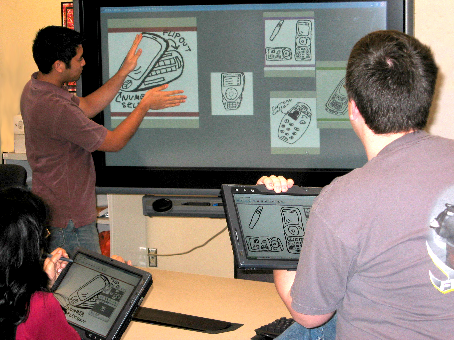
\includegraphics[width=\linewidth]{gfx/teamStormDisplayInteraction.png}
	\caption{Designer bei der Ausarbeitung von Konzepten mit \emph{Team Storm}.}
	\label{fig:teamStormDisplayInteraction}
\end{figure}

Skizzen, die von einem Teilnehmer aus seinem privaten Arbeitsbereich in den gemeinsamen Bereich gezogen werden, befinden sich standardmäßig im Ausstellungsmodus. Das bedeutet, dass alle Designer die Zeichnung sehen, sie positionieren und skalieren, jedoch nicht ändern können. Sollte der Urheber der Skizze nicht wünschen, dass Größe und Position von seinen Kollegen nicht verändert werden dürfen, so kann er den Zugriff sperren. Er kann die Zeichnung jedoch auch ganz freigeben, sodass nicht nur Skalierung und Position für die Kollegen veränderbar sind. Um eine Zeichnung vom gemeinsamen Bereich zu entfernen, zieht der Designer sie wieder zurück in seinen privaten Arbeitsbereich.

Designer können freigegebene Skizzen direkt auf der gemeinsamen Arbeitsfläche modifizieren, damit die anderen Teilnehmer die Änderungen live mitverfolgen können. Zusätzlich gibt es die Möglichkeit, sich eine private Kopie zu erstellen, die ohne Einsicht der anderen Teilnehmer editiert werden kann. Dadurch können Designs in mehreren Iterationen editiert und verfeinert werden. Die unterschiedlichen Versionen nebeneinander angereiht zeigen die Evolution einer bestimmten Idee.

Die an \emph{Team Storm} durchgeführte Studie \citep{Hailpern:2007p113} zeigt, dass Designer, die das erste Mal mit dem System arbeiteten, einen sehr einfachen und direkten Zugang zu dieser Groupware fanden. Es wurden sehr viele Ideen generiert und die Teilnehmer nutzten sehr stark die Features zur Organisation der Konzepte und Designs. Unterschiedliche Charaktere brachten unterschiedliche Arbeitsweisen zum Vorschein: einige Designer teilten offen jeden ihrer gezeichneten Striche mit, während andere es bevorzugten, Skizzen erst im privaten Bereich anzufertigen, um sie selbst zu evaluieren bevor sie sie herzeigten.

Die Gruppen nutzten das System auf sehr individuelle Art und Weise. Während manche hauptsächlich gemeinsam an einzelnen Designs arbeiteten, zogen andere es vor, parallel an verschiedenen Konzepten zu arbeiten, die dann gemeinsam evaluiert wurden.

Neben diesen positiven Eindrücken, kristallisierten sich auch einige mögliche Optimierungen des Systems heraus. Die Designer wünschten sich, Konzepte in Gruppen zu organisieren, die sie dann als Einheit positioniert, skaliert und hergezeigt hätten. Die Navigation wurde von vielen bei steigender Anzahl von Skizzen als ineffizient empfunden. Das System sah nur Scrolling und Zooming vor, die Teilnehmer wünschten sich hier weitere Möglichkeiten. Zusätzlich kam das Bedürfnis auf, andere digitale Artefakte (z. B. Bilder und Webseiten) einzubinden und dadurch Skizzen anzureichern.

\section{CSCW und Groupware}
>>Computer Supported Cooperative Work<< ist jene Wissenschaft, die sich der Erforschung von kooperativer Zusammenarbeit mehrerer Personen widmet, um folglich Applikationen und Systeme zur Verbesserung selbiger zu konzipieren \citep{Bannon:1990p244}. Der Fokus liegt darin, die Natur der kooperativen Arbeit besser zu verstehen und daraus Designkriterien abzuleiten, die es ermöglichen, effizientere Systeme zur Unterstützung dieses komplexen Prozesses zu entwickeln. 

\begin{figure}[bth]
	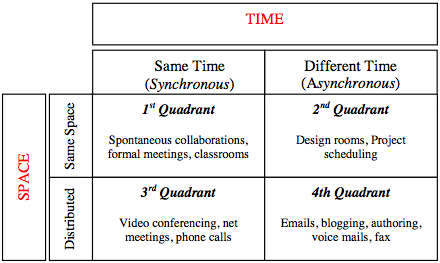
\includegraphics[width=\textwidth]{gfx/ramaCSCWQuadranten.png}
	\caption{Rama und Bishop \citep{Rama:2006p245} illustrieren in dieser Grafik die Unterteilung von CSCW in vier Kategorien, die sich durch ihre räumlichen und zeitlichen Eigenschaften unterscheiden. Der Faktor Zeit definiert, ob Zusammenarbeit in einer Gruppe synchron oder asynchron passiert und der Faktor Raum definiert, ob sie am selben oder an geographisch distanzierten Orten passiert.}
	\label{fig:ramaCSCW}
\end{figure}

Dem gegenüber steht der Begriff Groupware, auch bekannt als >>kollaborative Software<< \citep{Bannon:1990p244}, die mehreren Personen ermöglicht, gemeinsam am selben Projekt zu arbeiten. Groupware ist die technisch fokussierte Anwendung der Erkenntnisse, welche die Erforschung von CSCW hervorgebracht hat. Diese bestimmte Art von Software zielt darauf ab, gruppendynamische Prozesse zu vereinfachen und die Kommunikation innerhalb kooperierender Gruppen zu ermöglichen, beziehungsweise zu fördern. Der zusätzliche Koordinationsaufwand soll minimiert und das Lösen von Problemstellungen in Teams optimiert werden \citep{Rama:2006p245}. Gerlicher und Ansgar \citep{Gerlicher:2007p241} unterteilen Groupware in synchrone, asynchrone und multisynchrone Systeme.

\subsection{Weitere spezifische Systeme}

\emph{Anmerkung: \graffito{\(\clubsuit\)} Es folgen verschiedene kollaborative Systeme, die nicht unbedingt mit Skizzieren in Verbindung gebracht werden, aber das Prinzip von CSCW veranschaulichen.}


\subsection{Konzepte zur Kooperation am selben Ort}

Auf der Suche nach Konzepten, zur Förderung der kreativen Zusammenarbeit von Industriedesigner in gemeinsamen Meetings, halten Wang und Blevis \citep{Wang:2004p110} sich an die Methode des >>human centered design<<\footnote{Beim human centered design steht der potenzielle Benutzer eines Produktes im Mittelpunkt des Entwicklungsprozesses. Seine Aufgaben, Ziele, Fähigkeiten und Eigenschaften werden analysiert und gelten als Maßstab bei der Gestaltung des Produkts. Human centered design zielt darauf ab, möglichst benutzerfreundliche Produkte zu schaffen.} und führen zuerst eine ethnographische Studie an der Zielgruppe durch. Ausgehend von den so erlangten Erkenntnissen, entwickeln sie vier unterschiedliche Konzepte, die speziell darauf abzielen die konkrete Arbeitsweise der Industriedesigner zu unterstützen. Diese Konzepte sind aus technischer Sicht nicht unbedingt innovativ, dafür aber für ihre Zielgruppe besonders gut geeignet.

In ihrer Studie konzentrieren sich Wang und Blevis \citep{Wang:2004p110} darauf, die Interaktionen zwischen den Designern zu beobachten und nicht die Interaktion mit speziellen interaktiven Geräten. Ferner observieren die Forscher die verschiedenen nicht technologischen Artefakte und Geräte, sowie deren Orientierung und Gebrauchsweise, die bei der Zusammenarbeit zum Einsatz kommen. Davon ausgehend versuchen sie, möglichst ganzheitliche Konzepte zu entwickeln. Einen weiteren Fokus der Studie bildet das Identifizieren der Unterschiede zwischen privaten und gemeinsamen Arbeitsbereichen im kollaborativen Prozess.

\subsubsection{Designkriterien}

Die folgenden Punkte haben sich aus dieser Studie als relevant herauskristallisiert und fließen als Designkriterien in die danach vorgestellten Konzepte mit ein.

\begin{itemize} 
	\item{\emph{Sitzordnung}}\\
	Augenkontakt ist eine der wichtigsten Formen der Kommunikation bei der Zusammenarbeit in Gruppen. Daher bevorzugen die Teilnehmer, um einen Tisch herum zu sitzen, damit sie alle direkt ansehen können.
	\item{\emph{Reichweite}}\\
	Es ist besonders wichtig, dass alle Objekte für jeden Teilnehmer in Reich- und Sichtweite liegen. Durch die Interaktion mit den Objekten, können Teilnehmer sich in den Fokus der Aufmerksamkeit stellen und besser kommunizieren. Rechteckige Tische bieten Nachteile für jene Personen, die an den Ecken sitzen, weshalb runde Tische bevorzugt werden.
	\item{\emph{Simultanität}}\\
	Häufig interagieren mehrere Benutzer gleichzeitig mit den Objekten im Arbeitsbereich und fast immer sind viele verschiedene Artefakte präsent. Ein gutes Konzept muss daher diese Gleichzeitigkeit gewährleisten können, um die Effizienz durch paralleles Arbeiten nicht zu gefährden.
	\item{\emph{Gebrauch physischer Objekte}}\\
	In der direkten face-to-face Kommunikation bevorzugen Personen physische Objekte, da sie im direkten Gespräch effizienter genutzt werden können als digitale Objekte.
	\item{\emph{Große Arbeitsflächen, viele Blätter, Wiederfindung und Vergleich}}\\
	Designer benötigen sehr große Arbeitsflächen im Zuge der kreativen Ideenfindung. Sie verteilen die verschiedenen Konzepte darauf und Anordnung und Gruppierung spielen eine wichtige Rolle. Um einzelne Ideen leichter wieder zu finden und untereinander zu vergleichen, zeichnen sie üblicherweise nur eine davon auf ein gesamtes Blatt Papier.
	\item{\emph{Privatsphäre}}\\
	Die Teilnehmer benötigen private Arbeitsbereiche, in denen sie Konzepte ausarbeiten und selbst evaluieren können, und sie brauchen gemeinsame Arbeitsbereiche, auf denen sie alle zusammen die Entwicklung vorantreiben.
	\item{\emph{Ausrichtung von Objekten}}\\
	Die Ausrichtung von Objekten ist Teil der Privatsphäre. Sind Objekte zu einer bestimmten Person hin ausgerichtet, so gelten diese als privat, wenn sie hingegen zur Gruppe hin gerichtet sind, finden alle Teilnehmer einen Zugang.
\end{itemize}

\begin{figure}[bth]
	\myfloatalign
	\subfloat[\emph{Multi-user ClearBoard mit MiniNavigator}]{
		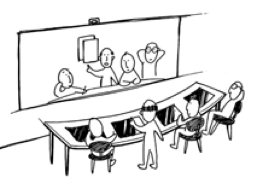
\includegraphics[width=.6\textwidth]{gfx/wangClearBoardConcept.png}
	} 
	\quad
	\subfloat[\emph{3D-Navigator}]{
		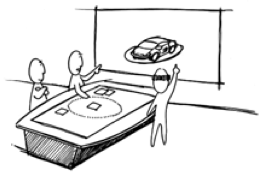
\includegraphics[width=.6\textwidth]{gfx/wang3DNavigatorConcept.png}
	}
	\quad
	\subfloat[\emph{ConverTable}]{
		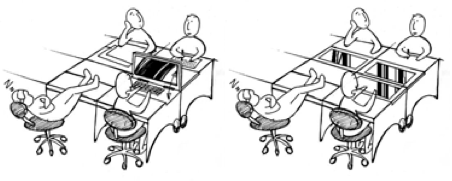
\includegraphics[width=\textwidth]{gfx/wangConverTableConcept.png}
	}
	\quad
	\subfloat[\emph{More is more}]{
		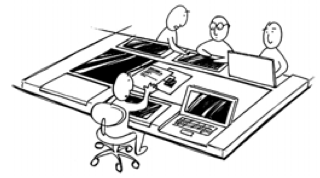
\includegraphics[width=.6\textwidth]{gfx/wangMoreIsMoreConcept.png}
	}
	\caption{Vier verschiedene Konzepte wurden von Wang und Blevis \citep{Wang:2004p110} entwickelt. Sie berücksichtigen die Designkriterien, die zuvor in einer Studie mit Industriedesignern ermittelt wurden.}
	\label{fig:wangConcepts}
\end{figure}

Auf diesen Erkenntnissen aufbauend, haben Wang und Blevis \citep{Wang:2004p110} vier verschiedene Konzepte entwickelt, die kollaborative Meetings von Industriedesignern unterstützen. 

\subsubsection{Multi-user ClearBoard mit MiniNavigator}

Das \emph{Multi-user ClearBoard mit MiniNavigator} (\autoref{fig:wangConcepts}) ist eine Weiterentwicklung des von Hiroshi Ishii et al. konzipierten \emph{ClearBoard}\citep{Ishii:1994p243}. Alle Benutzer sitzen an einem Tisch und vor ihnen wird ein großes Bild auf die Wand projiziert. Auf diesem werden die digitale Arbeitsfläche und ein Videobild der Teilnehmer übereinander gelegt, sodass jeder die Gestiken und Mimiken der anderen Kollegen, als auch die digitalen Artefakte sehen kann. Zusätzlich verfügt jeder Benutzer über ein eigenes Touch-Display. Auf diesem wird ebenfalls dasselbe Bild wie an der Wand angezeigt und dient zur Interaktion mit den digitalen Elementen auf der Arbeitsfläche.

\subsubsection{3-D Navigator}

Das \emph{3-D Navigator} Konzept ermöglicht den Designern dreidimensionale Modelle aus verschiedenen Perspektiven zu betrachten, indem sie natürliche Gesten verwenden. Das System besteht aus einem großen, berührungsempfindlichen Tabletop-Display\footnote{Tabletop-Display bezeichnet einen großen Flachbildschirm, der in eine Tischplatte integriert ist. In bestimmten Fällen ist dieser auch berührungsempfindlich und dient nicht nur der Ausgabe, sondern auch der Eingabe.} und einem Projektor, der ein großes Bild auf eine Wand projiziert. Das Tabletop-Display dient als Schnittstelle und zeigt alle verschiedenen dreidimensionalen Modelle in Handflächengröße an. Diese können von den Benutzern mit dem Finger verschoben werden. Damit ein Modell vom Projektor auf die Wand projiziert wird, muss es auf dem Tabletop-Display in den in der Mitte dargestellten Kreis geschoben werden. 

\subsubsection{More is more}

\emph{More is more} berücksichtigt das Bedürfnis der Designer nach einer großen, gemeinsamen Arbeitsfläche, als auch jenes nach privaten Bereichen zur eigenständigen Entwicklung von Konzepten und Ideen. \autoref{fig:wangConcepts} zeigt die geschickte Anordnung von sechs Displays auf einem Tisch, die einzeln in eine vertikale oder horizontale Position gebracht werden können. Im aufgerichteten Zustand stellt ein Display einen privaten Arbeitsbereich dar. Designer können so für sich selbst arbeiten. Indem sie dann das Display hinunter klappen, wechseln sie in einen halb privaten Modus, denn Kollegen, die neben oder vor ihnen sitzen, können nun das Display sehen und mitarbeiten. Andere Personen, die nicht so nah sitzen haben jedoch noch keine Einsicht. Damit jeder teilhaben kann, gibt es im mittleren Bereich des Tisches ein gemeinsames, für alle sichtbares Display. Die Designer können ihre Modelle und Konzepte dort hin ziehen und für alle zugänglich machen.

\subsubsection{ConverTable}

Mit dem \emph{ConverTable} schlagen Wang und Blevis ein weiteres Konzept vor, das es sehr vereinfacht, zwischen privatem und gemeinsamen Arbeitsmodus zu wechseln. Designer können \emph{ConverTable} als einfachen Tisch nutzen und mit physischen Objekten und Artefakten darauf arbeiten. Bei Bedarf bringen sie das integrierte Display in eine vertikale Position und schaffen sich somit Zugang zu virtuellen Modellen. Ausgestattet mit Rädern, ist der \emph{ConverTable} ein höchst mobiles und elektronisch raffiniertes Möbelstück, das auch für spontanes Zusammenarbeiten sehr gut geeignet ist.

\section*{Zusammenfassung}
lorem ipsum

%*****************************************
%*****************************************
%*****************************************
%*****************************************
%*****************************************
